
\documentclass[10pt,conference]{IEEEtran}

\usepackage{booktabs} % For formal tables
%\usepackage{pifont}
\usepackage{multirow}


\usepackage{graphicx}
\usepackage{caption}

% *** SUBFIGURE PACKAGES ***
\usepackage{subfig}

\usepackage{blindtext}
\usepackage{adjustbox}
\usepackage{multirow}
\usepackage{color}
\usepackage{booktabs}
\usepackage{tabularx}
\usepackage{colortbl}
\usepackage{bbding}
\usepackage{tikz}
\usepackage{listings}
\usepackage{etoolbox}
\usepackage{subfig}

\usepackage{url}
\usepackage{setspace}
%\usepackage{enumitem}
\usepackage[british,english]{babel}


%\usepackage[caption=false,font=footnotesize]{subfig}


\newcommand{\circled}[2][]{\tikz[baseline=(char.base)]
    {\node[shape = circle, draw, inner sep = 1pt]
    (char) {\phantom{\ifblank{#1}{#2}{#1}}};%
    \node at (char.center) {\makebox[0pt][c]{#2}};}}
\robustify{\circled}


\newcommand\FIXME[1]{\textcolor{red}{FIX:}\textcolor{red}{#1}}

\makeatletter
\def\@IEEEsectpunct{.\ \,}
\def\paragraph{\@startsection{paragraph}{4}{\z@}{1.5ex plus 1.5ex minus 0.5ex}%
{0ex}{\normalfont\normalsize\sffamily\bfseries}}


\patchcmd{\@maketitle}
  {\addvspace{0.2\baselineskip}\egroup}
  {\addvspace{-1\baselineskip}\egroup}


\makeatother

\newcommand{\cparagraph}[1]{\vspace{1mm}\noindent \textbf{#1}}



\newcommand{\topone} {{top-1}\xspace}
\newcommand{\topfive} {{top-5}\xspace}
\newcommand{\DNN} {\texttt{DNN}\xspace}
\newcommand{\DNNs} {\texttt{DNNs}\xspace}
\newcommand{\CNN} {\texttt{CNN}\xspace}
\newcommand{\RNN} {\texttt{RNN}\xspace}
\newcommand{\RNNs} {\texttt{RNNs}\xspace}
\newcommand{\CNNs} {\texttt{CNNs}\xspace}
\newcommand{\NN} {\texttt{KNN}\xspace}
\newcommand{\nNN} {\texttt{NN}\xspace}
\newcommand{\SVM} {\texttt{SVM}\xspace}
\newcommand{\DT} {\texttt{DT}\xspace}



\begin{document}

\title{\LARGE \emph{To Compress, or Not to Compress:} Understanding Deep Learning Model Compression for Embedded Inference}

\author{\IEEEauthorblockN{Qing Qin\IEEEauthorrefmark{3},
         Jie Ren\IEEEauthorrefmark{2}, Jialong Yu\IEEEauthorrefmark{3}, Lu Yuan\IEEEauthorrefmark{3}, Ling Gao\IEEEauthorrefmark{3}, Jie
         Zheng\IEEEauthorrefmark{3},
         Jianbin Fang\IEEEauthorrefmark{4}, Yansong Feng\IEEEauthorrefmark{5},
         Zheng Wang\IEEEauthorrefmark{1}}

 \IEEEauthorblockA{\IEEEauthorrefmark{3} Northwest University, China, \IEEEauthorrefmark{2} Shaanxi Normal University, China, \IEEEauthorrefmark{4} National University of Defense Technology, China}
 \IEEEauthorblockA{\IEEEauthorrefmark{5} Peking University, China, \IEEEauthorrefmark{1} Lancaster University, United Kingdom}

 }

\maketitle


\begin{abstract}
The recent advances in deep neural networks (\DNNs) make them attractive for embedded systems. However, it can take a long time for DNNs
to make an inference on resource-constrained computing devices. Model compression techniques can address the computation issue of deep
inference on embedded devices. This technique is highly attractive, as it does not rely on specialized hardware, or
computation-offloading that is often infeasible due to privacy concerns or high latency. However, it remains unclear how model
compression techniques perform across a wide range of \DNNs. To design efficient embedded deep learning solutions, we need to understand
their behaviors. This work develops a quantitative approach to characterize model compression techniques on a representative embedded
deep learning architecture, the NVIDIA Jetson Tx2. We perform extensive experiments by considering 11 influential neural network
architectures from the image classification and the natural language processing domains. We experimentally show that how two mainstream
compression techniques, data quantization and pruning, perform on these network architectures and the implications of compression
techniques to the model storage size, inference time, energy consumption and performance metrics. We demonstrate that there are
opportunities to achieve fast deep inference on embedded systems, but one must carefully choose the compression settings. Our results
provide insights on when and how to apply model compression techniques and guidelines for designing efficient embedded deep learning
systems.
\end{abstract}


\begin{IEEEkeywords}
Deep learning, embedded systems, parallelism, energy efficiency
\end{IEEEkeywords}

\section{Introduction}
In recent years, deep learning has emerged as a powerful tool for solving problems that were considered to be difficult in the past. It has
demonstrated impressive results on tasks like object recognition~\cite{donahue14,he2016deep}, facial
recognition~\cite{parkhi2015deep,sun2014deep}, speech processing~\cite{pmlrv48amodei16}, and machine translation~\cite{bahdanau2014neural}.
While many of these tasks are also important on mobiles and the Internet of Things (IoT), existing solutions are often
computation-intensive and require a large amount of resources for the model to operate. Performing deep inference\footnote{Inference in
this paper refers to apply a pre-trained model on an input to obtain the corresponding output. This is different from statistical
inference.} on embedded devices can lead to long runtimes and the consumption of abundant amounts of resources, including CPU, memory, and
power, even for simple tasks~\cite{CanzianiPC16}. Without a solution,
 the hoped-for advances on embedded sensing will not arrive.


Numerous approaches have been proposed to accelerate deep inference on embedded devices. These include designing specialize hardware to
reduce the computation or memory latency~\cite{}, compressing a pre-trained model to reduce its storage and memory footprint as well as
computational requirements~\cite{}, and offloading some, or all, computation to a cloud
server~\cite{Kang2017neurosurgeon,teerapittayanon2017distributed}. Compared to specialized hardware, software-based model compression
techniques have the advantage of being readily deployable on commercial-off-the-self hardware and compared to computation offloading, model
compression enables on-device inference which in turn allows faster response time and has less privacy concerns. These advantages make
model compressions attractive on existing hardware platform where computation offloading is not feasible.


However, model compression is not a free lunch as it comes at the cost of loss in prediction accuracy~\cite{}. This means that one must
carefully choose the model compression technique and its parameters to effectively trade precision for computation and resource
requirements. Furthermore, as we will show in this paper, the reduction in the model size does not necessarily translate into faster
inference time. Because a model compression technique is not always beneficial, it is important to understand when and how to apply a
 technique.

In this paper, we aim to understand model compression techniques for embedded inference. Having this knowledge allows not only better
deployment of computation-intensive models on mobile and IoT devices, but also designing more efficient architectures for models and
hardware acceleration.

In this work, we conducted extensive experiments to evaluate two mainstream model compression techniques, pruning~\cite{Li2016Pruning} and data
quantization~\cite{Gong2014Compressing}. We apply model compression techniques to the image classification domain, an area where deep learning has made
impressive breakthroughs and a rich set of pre-trained models are available. We evaluate our approach on the NVIDIA Jetson TX2 embedded
deep learning platform and consider a wide range of influential DNN models. Our experiments are performed using the 50K images from the
ImageNet ILSVRC 2012 validation dataset.

We show that while there may be significant gain for choosing the right compression technique and parameters, mistakes can seriously hurt
the performance. We show how different model compression techniques and parameters affect the inference time, model storage requirement and
the prediction accuracy. As a result, our work provides insights on when and how to apply deep learning model compression techniques on
embedded devices.

The main contributions of this paper are two folds:

\begin{itemize}
\item We present an extensive study to characterize and understand how two popular model compression techniques perform on a
    representative embedded deep learning platform;
\item Our work offers insights on when and how to apply compression techniques for embedded deep inference.
\end{itemize}

\begin{figure*}[!t]
\centering
\subfloat[][Model size]{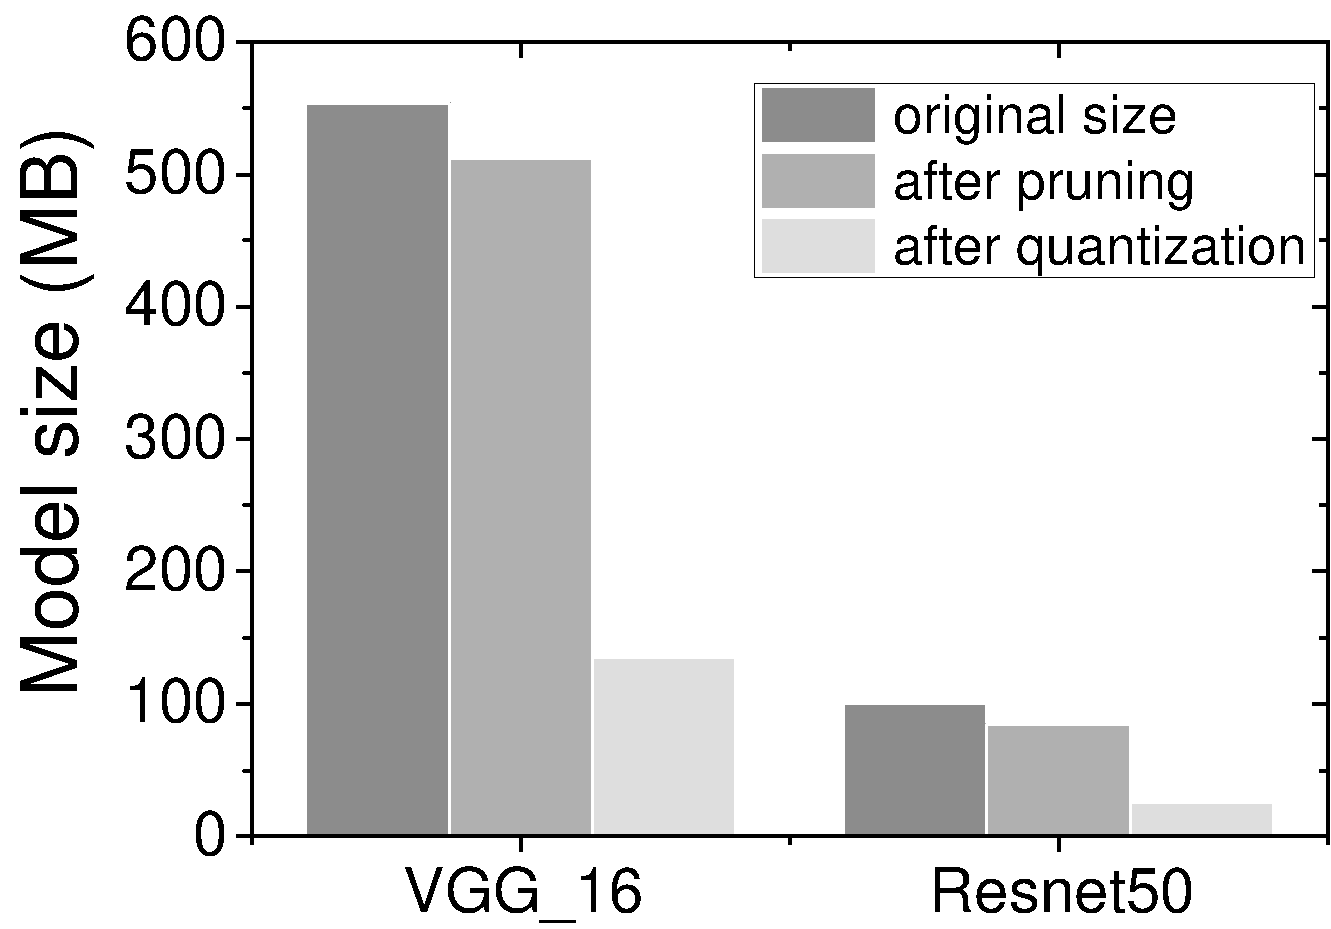
\includegraphics[width=0.23\textwidth]{figure/motivation_size.pdf}}
\hfill
\subfloat[][Inference time]{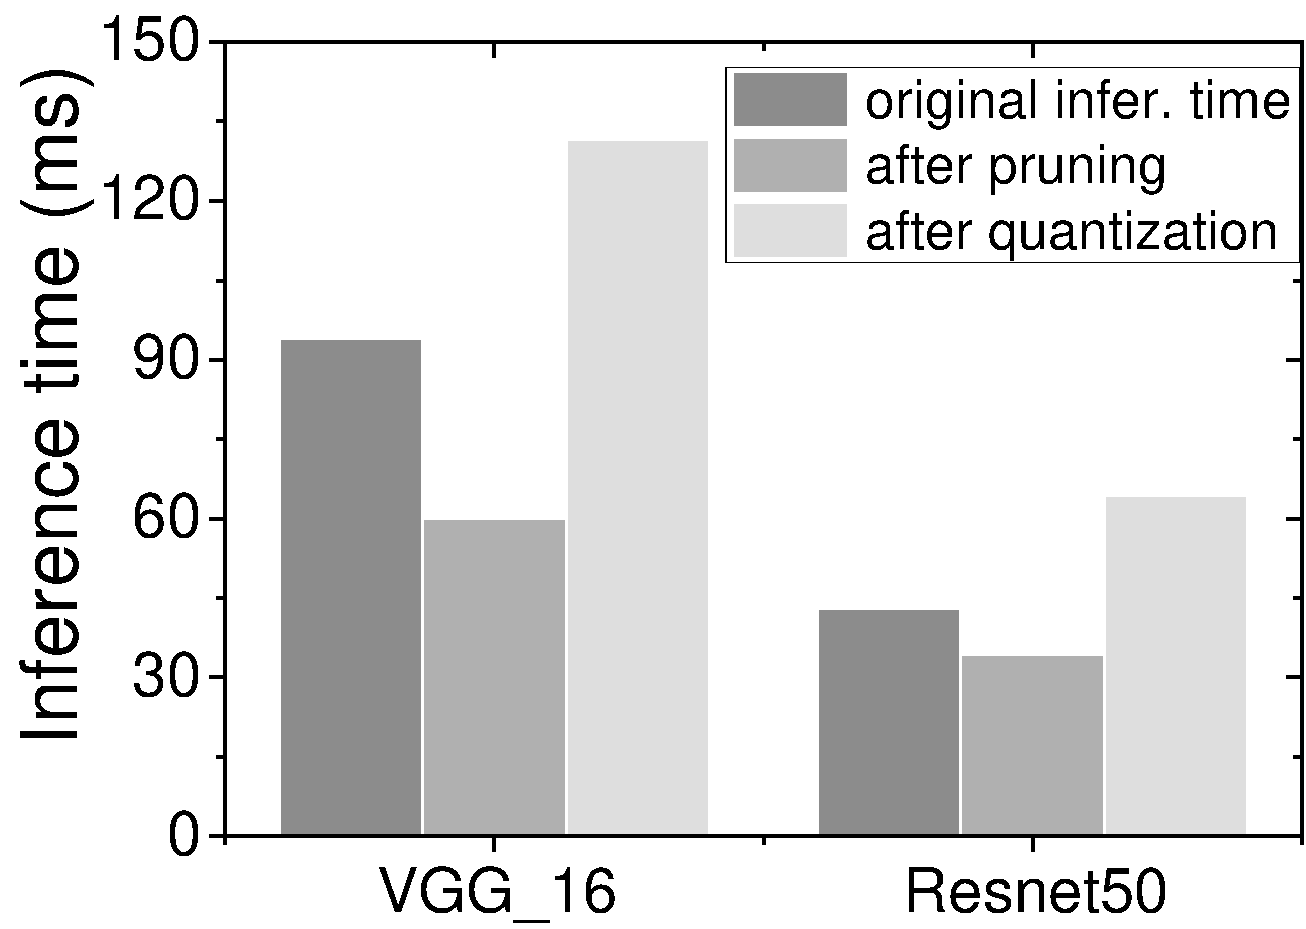
\includegraphics[width=0.23\textwidth]{figure/motivation_time.pdf}}
\hfill
\subfloat[][Energy consunption]{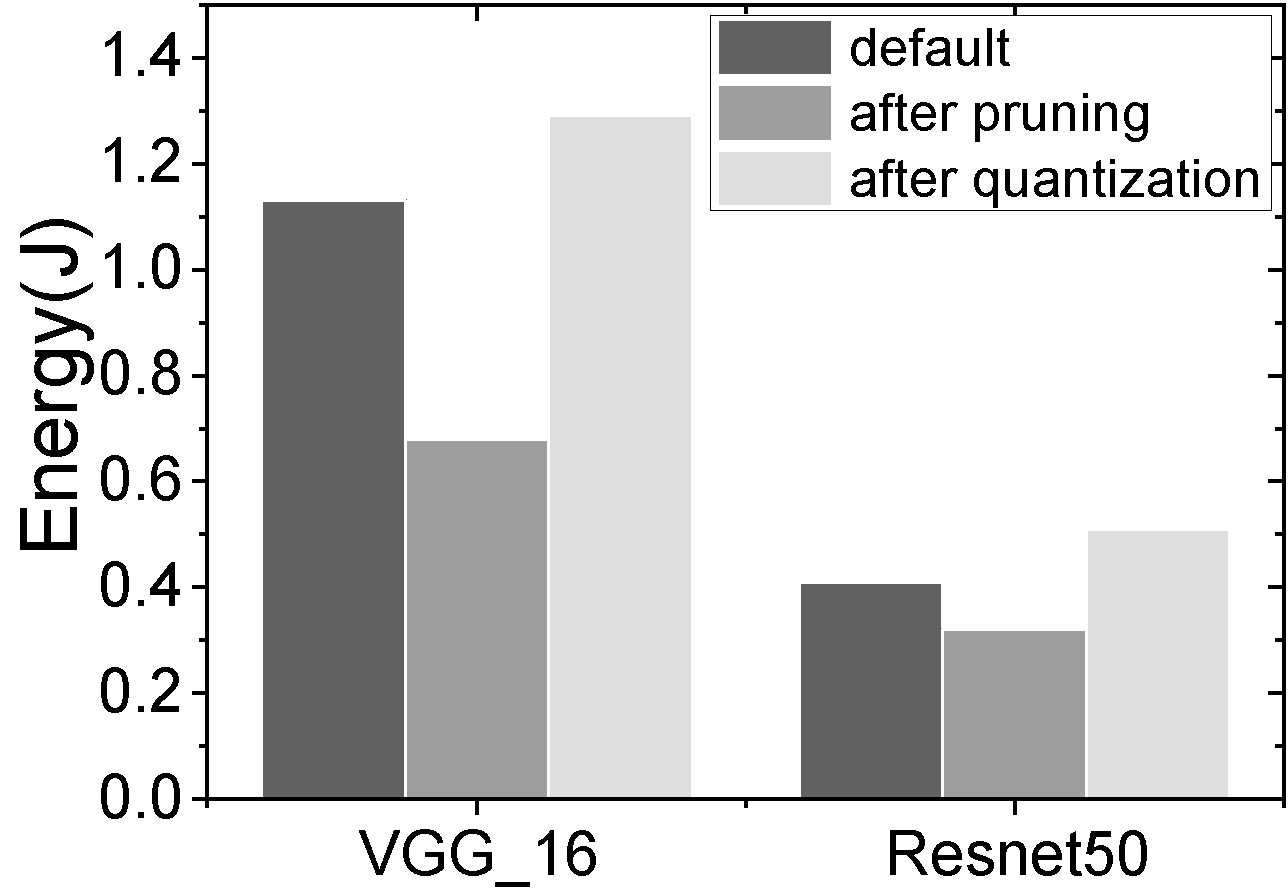
\includegraphics[width=0.23\textwidth]{figure/motivation_energy.pdf}}
\hfill
\subfloat[][Accuracy]{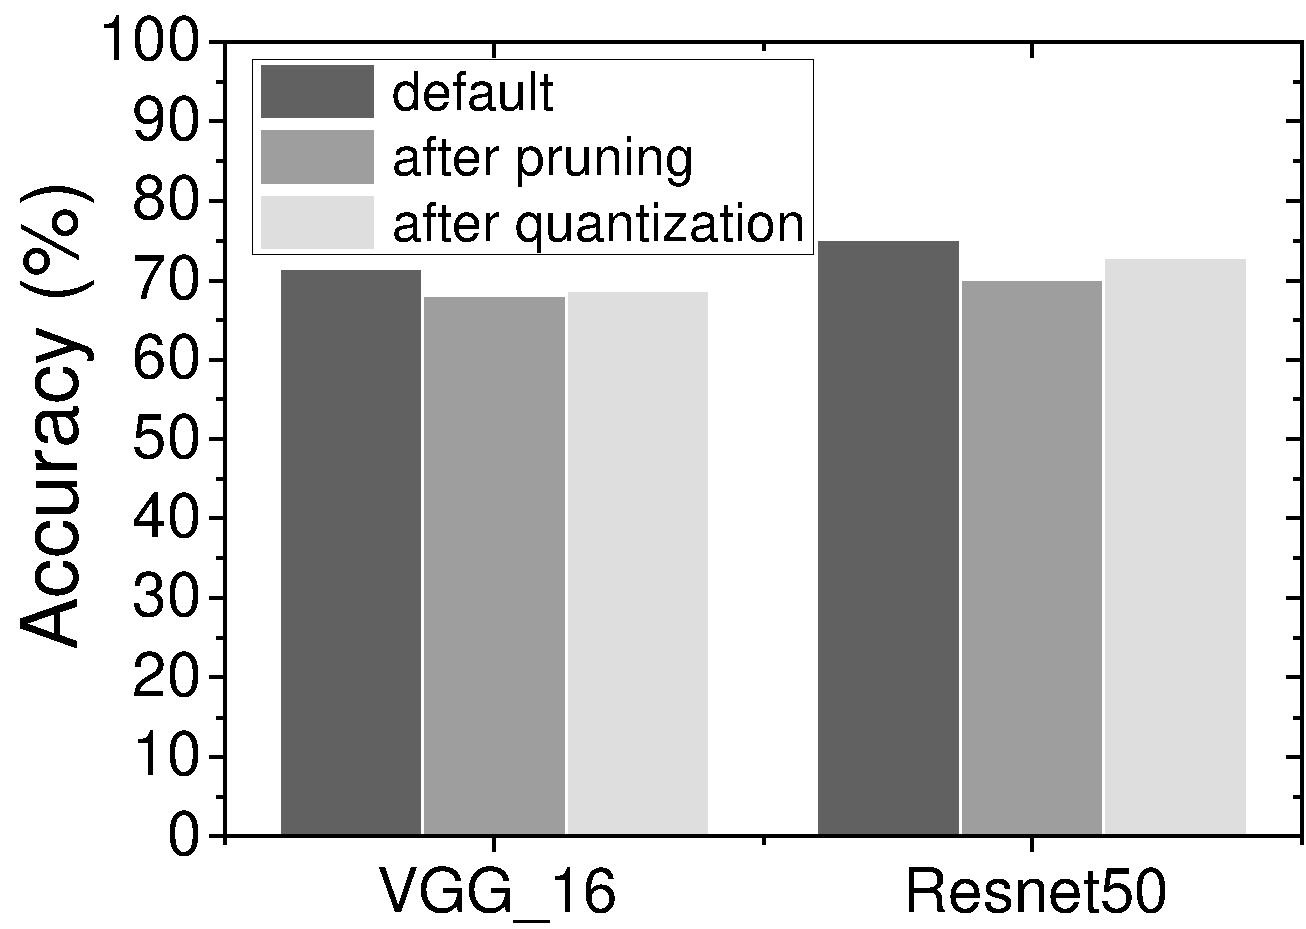
\includegraphics[width=0.23\textwidth]{figure/motivation_accuracy.pdf}}
\hfill
\caption{The achieved model size (a) inference time (b) energy consumption (c) and accuracy (d) before and after the compression by \quantization and \pruning.
The compression technique to use depends on the optimization target.}
\label{fig:motivation}
\end{figure*}

\section{Background and Motivation}
\subsection{Background}
In this work, we consider two commonly used model compression techniques, described as follows.

\cparagraph{Pruning.} This technique removes less important parameters from a trained network. Pruning ranks the neurons in the network
according how much the neuron contribute, it then removes the low ranking neurons to reduce the model size. Care must be taken to not
remove too many neurons to significantly damage the accuracy of the network.

\cparagraph{Data quantization.} This technique reduces the number of bits used to store the weights of a network, e.g., using 8-bit to
represent a 32-bit floating point number. In this work, we apply data quantization to convert a pre-trained floating point model into a
fixed point model without re-training. We choose to use an 8-bit representation as it is the most common fixed point data quantization
approach~\FIXME{\cite{}}.



\subsection{Motivation}
Choosing the right compression technique is non-trivial. As a motivation example, consider applying two widely used model compression
techniques, \pruning~\cite{manessi2017automated} and \dquantization~\cite{han2015deep}, to two influential \CNN models, \texttt{VGG\_16} 	and
\texttt{Resnet\_50}. Our evaluation platform is a NVIDIA Jetson TX2 embedded deep learning platform (see Section~\ref{sec:platform}).

\cparagraph{Setup.} We apply the compression technique to the pre-trained model (which has been trained on the ImageNet ILSVRC 2012
training dataset~\cite{imagenet2012}). We then test the original and the compressed models on ILVRSC 2012 validation set which contains 50k images.
We use pruning and quantization to compress two typical models \texttt{VGG\_16} and \texttt{Resnet 50},
and the loss of accuracy for pruning and quantization are less than 5\%,and 3\% respectively.
We use the GPU for
inferencing.

\cparagraph{Motivation Results.} Figure~\ref{fig:motivation} compares the model size, inference time and accuracy after applying model
compression. By removing some of the pathways of the network, \pruning is able to reduces the inference time and
energy consumption by 28\% and 22.5\%, respectively. However, it offers
little saving in storage size because network weights still deaminate the model size. By contrast, by using a few number of bits to
represent the weights, \quantization significantly reduces the model storage size by 75\%. However, the reduction in the model size does
not translate to faster inference time and fewer energy consumption; 
on the contrary, the inference time and energy increase by 1.41x and 1.19x respectively. 
%This is because the quantized graph adds a subgraph which containing the conversion function, 
%and converts 8 bits to 32 bits as the input of the output layer to ensure the accuracy of the output layer.
%Although the instantaneous power is reduced, the more energy is caused by the increased inference time.
This is because the sparsity in network
weights brought by \quantization leads to irregular computation which causes poor GPU performance~\cite{}. 
Applying both compression
techniques has modest impact on the prediction accuracy, on average, less than 5\%. This suggests that both techniques can be profitable.

\cparagraph{Lessons Learned.} This example shows that the compression technique to use depends on what to be optimized for. If storage
space (e.g., RAM and disk) is a limiting factor, \quantization could be used, but a more powerful processor unit is required to achieve
quick on-device inference. If faster on-device turnaround time is a priority, \pruning can be employed but it would require sufficient
memory resources to store the model parameters.  Since offloading the computation into the cloud is often infeasible due to privacy
concerns, high latency, or the lack of connectivity, there is a need to understand the pros and cons of model compression techniques for
embedded deep learning. This work provides an extensive study to characterize the benefit and cost of commonly used deep learning
compression techniques on embedded systems.

\section{Experimental Setup \label{sec:setup}}
\subsection{Platform and Models\label{sec:platform}}
%Describe hardware
\cparagraph{Hardware.} Our experimental platform is a NVIDIA Jetson TX2 embedded platform. The system has a 64~bit dual-core Denver2 and a
64~bit quad-core ARM Cortex-A57 running at 2.0~Ghz, and a 256-core NVIDIA Pascal GPU running at 1.3~Ghz. The board has 8~GB of LPDDR4 RAM
and 96~GB of storage (32~GB eMMC plus 64~GB SD card).


%Describe software
\cparagraph{System Software.} We run the Ubuntu 16.04 operating system with Linux kernel v4.4.15. We use Tensorflow v.1.6, cuDNN (v6.0) and
CUDA (v8.0.64).


\cparagraph{Deep Learning Models.} We consider \FIXME{14} pre-trained \CNN models for image recognition from the TensorFlow-Slim
library~\cite{silberman2013tensorflow}. The models are built using TensorFlow and trained on the ImageNet ILSVRC 2012 training set.


\subsection{Evaluation Methodology \label{sec:method}}


\cparagraph{Evaluation Metrics} We consider the following metrics:

%\vspace{-2mm}
\begin{itemize}
\item \emph{\textbf{Inference time} (lower is better)}. Wall clock time between a model taking in an input and producing an output,
    excluding the model load time.

\item \emph{\textbf{Energy consumption} (lower is better)}. The energy used by a model for inference.  We deduct the static power used by
    the hardware when the system is idle.

\item \emph{\textbf{Accuracy} (higher is better)}. The ratio of correctly labeled images to the total number of testing images.

\item \emph{\textbf{Precision} (higher is better)}. The ratio of a correctly predicted images to the total number of images that are
    predicted to have a specific object. This metric answers e.g., ``\emph{Of all the images that are labeled to have a cat, how many
    actually have a cat?}".

\item \emph{\textbf{Recall} (higher is better)}. The ratio of correctly predicted images to the total number of test images that belong
    to an object class. This metric answers e.g., ``\emph{Of all the test images that have a cat, how many are actually labeled to have a
    cat?}".

\item \emph{\textbf{F1 score} (higher is better)}.  The weighted average of Precision and Recall, calculated as $2\times\frac{Recall
    \times Precision} {Recall + Precision}$. It is useful when the test datasets have an uneven distribution of object classes.

\item \emph{\textbf{BLUE}} {higher is better}. \FIXME{Explain blue here!}

\end{itemize}

\cparagraph{Performance Report.}  To collect inference time and energy consumption, we run each model on each input repeatedly until the
95\% confidence bound per model per input is smaller than 5\%. In the experiments, we exclude the loading time of the \CNN models as they
only need to be loaded once in practice. To measure energy consumption, we developed a lightweight runtime to take readings from the
on-board energy sensors at a frequency of 1,000 samples per second. We then matched the energy readings against the time stamps of model
execution to calculate the energy consumption.

\begin{figure*}[!t]
\centering
\subfloat[][Model size]{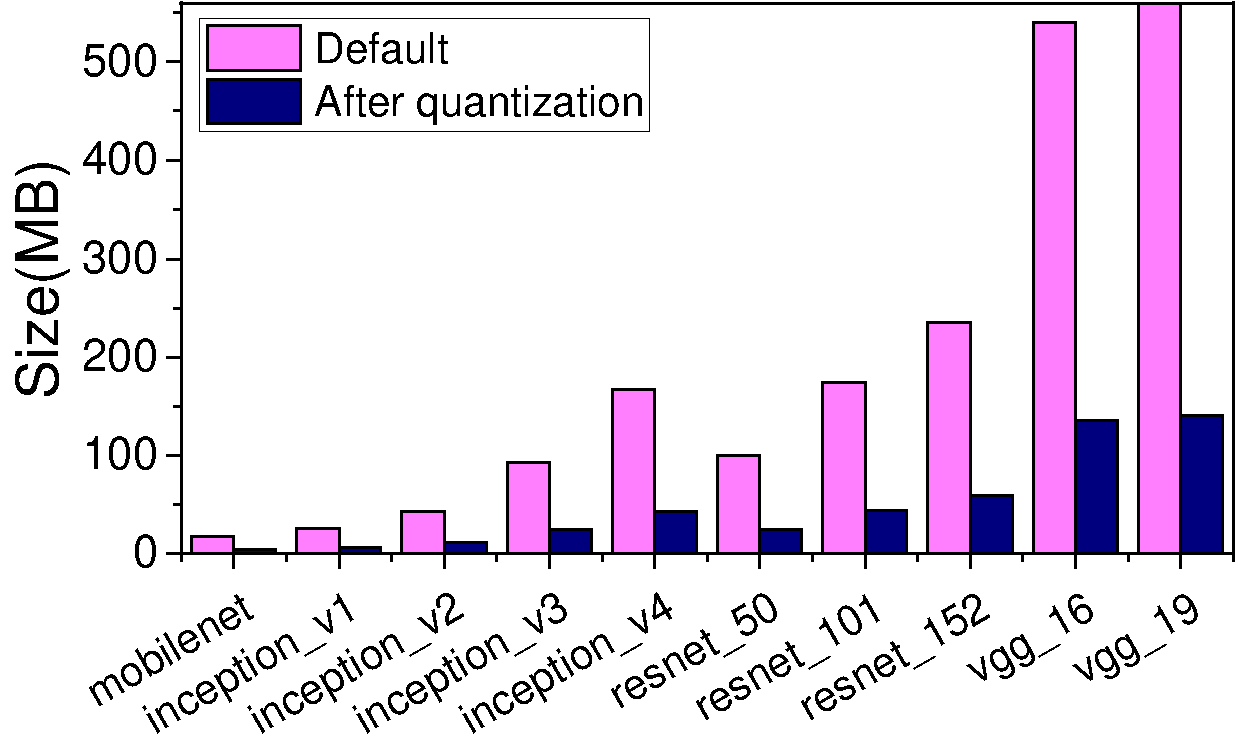
\includegraphics[width=0.33\textwidth]{figure/quan_size.pdf}}
\hfill
\subfloat[][Inference time]{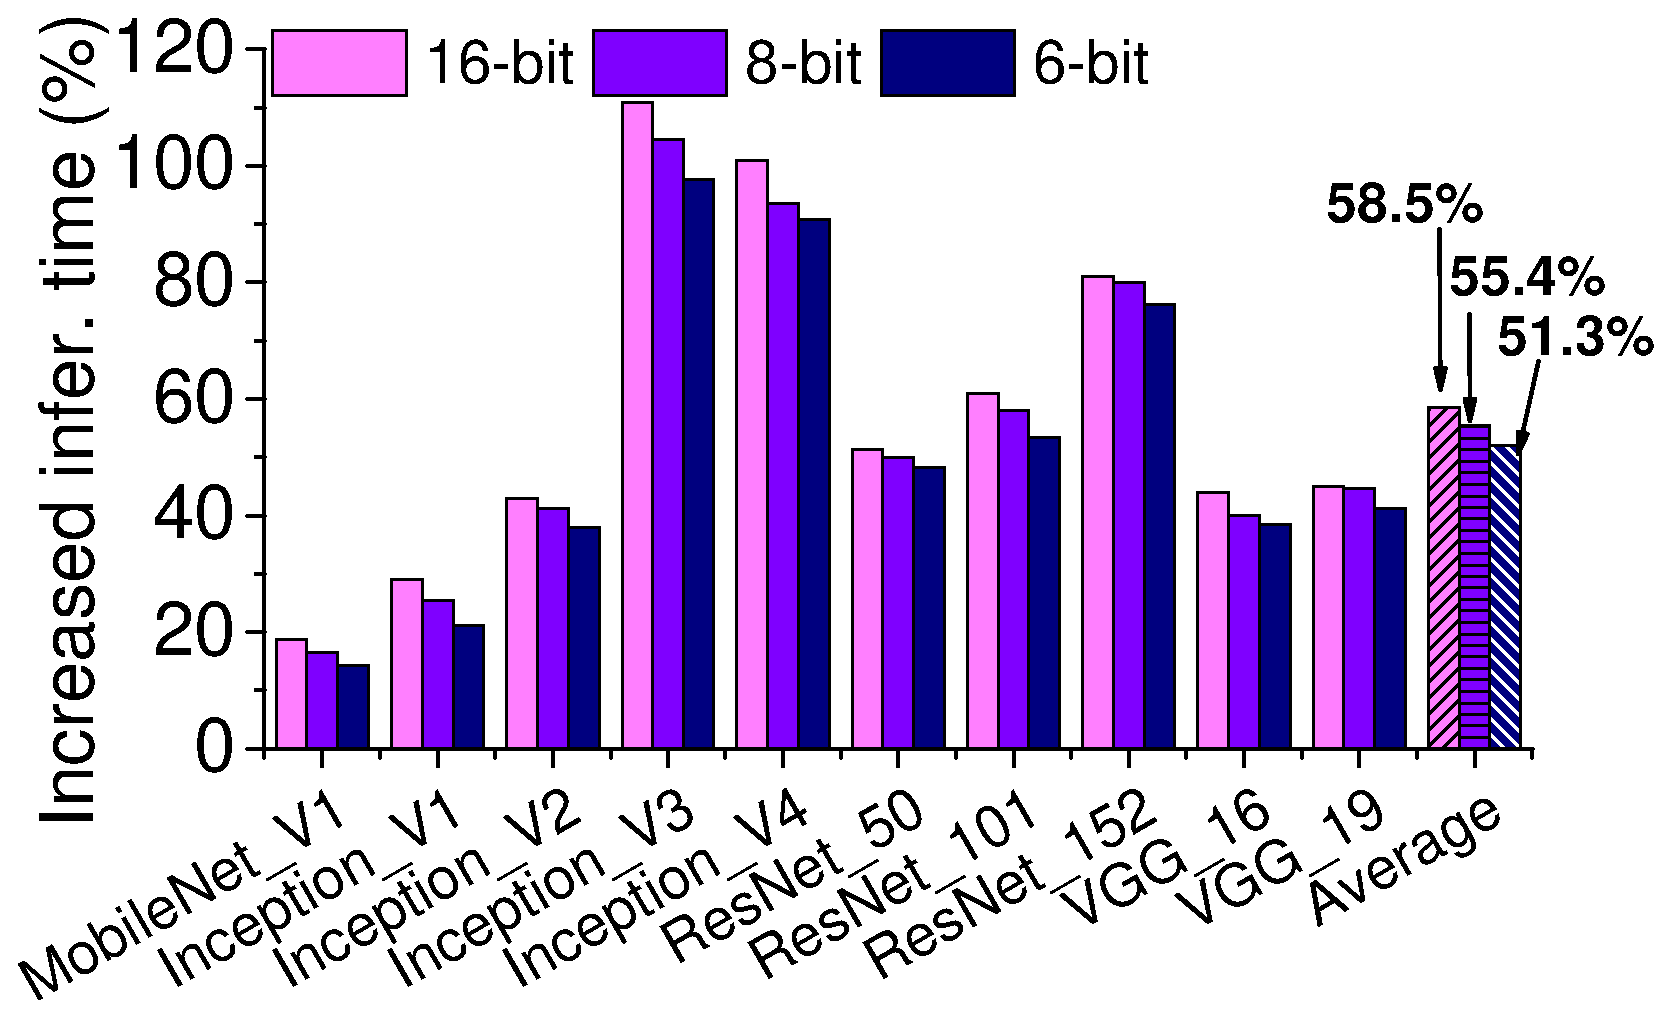
\includegraphics[width=0.34\textwidth]{figure/quan_time2.pdf}}
\hfill
\subfloat[][Accuracy]{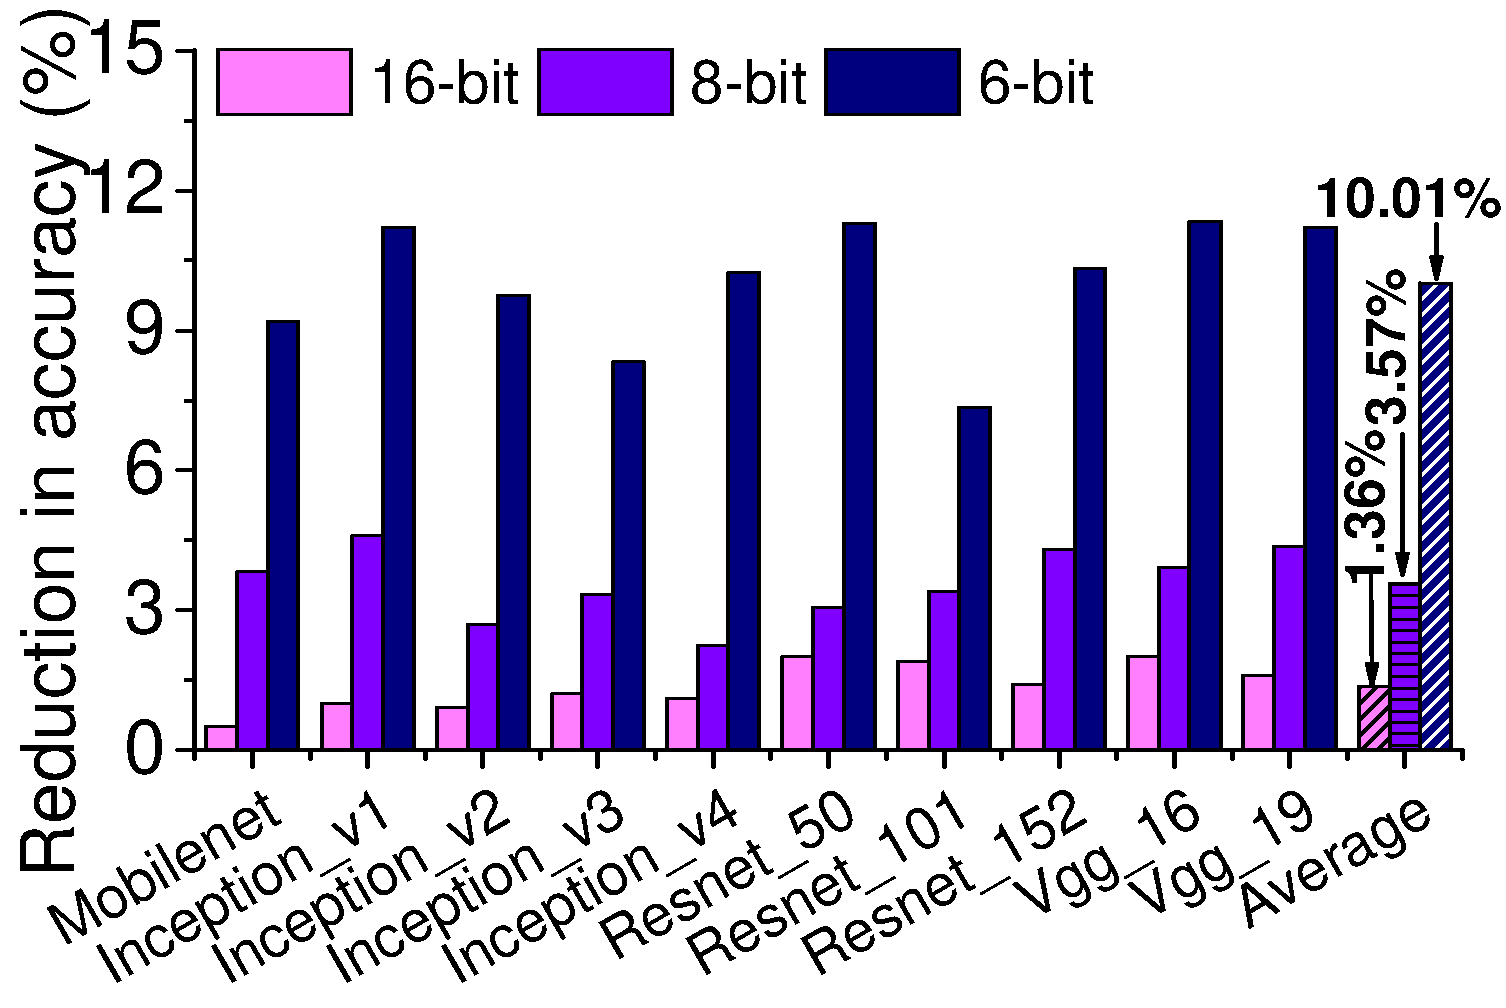
\includegraphics[width=0.32\textwidth]{figure/quan_acc3.pdf}}
\hfill
\subfloat[][Power consumption]{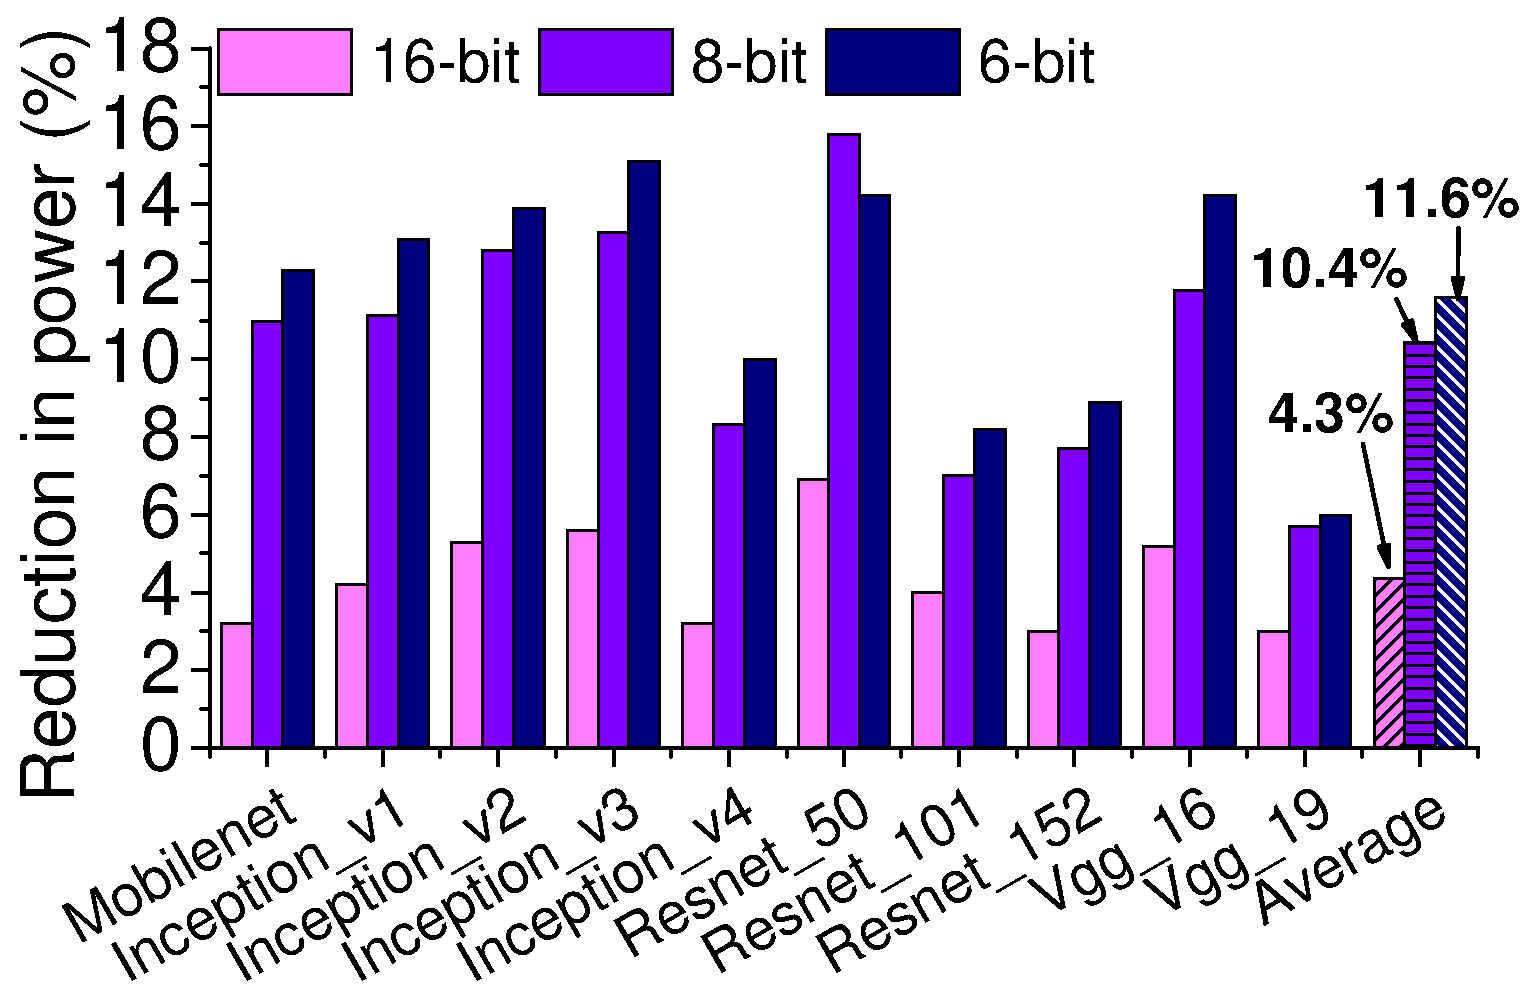
\includegraphics[width=0.33\textwidth]{figure/quan_power2.pdf}}
\hfill
\subfloat[][Energy consumption]{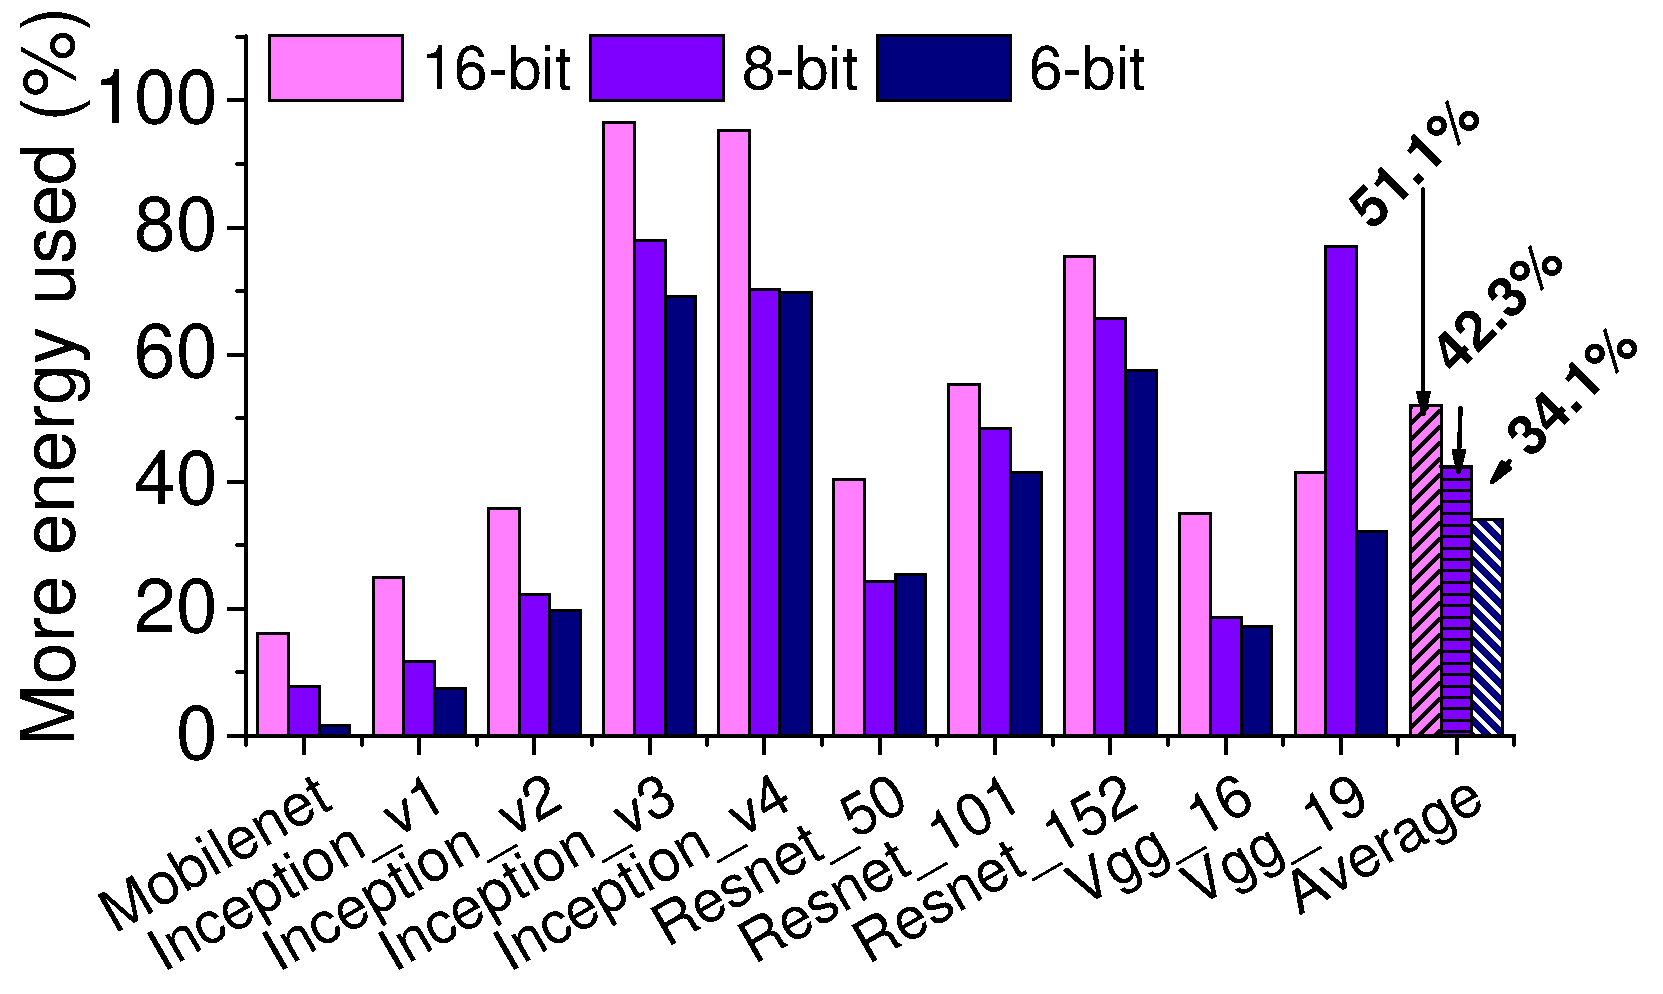
\includegraphics[width=0.34\textwidth]{figure/quan_energy2.pdf}}
\hfill
\subfloat[][precision, recall and F1 score]{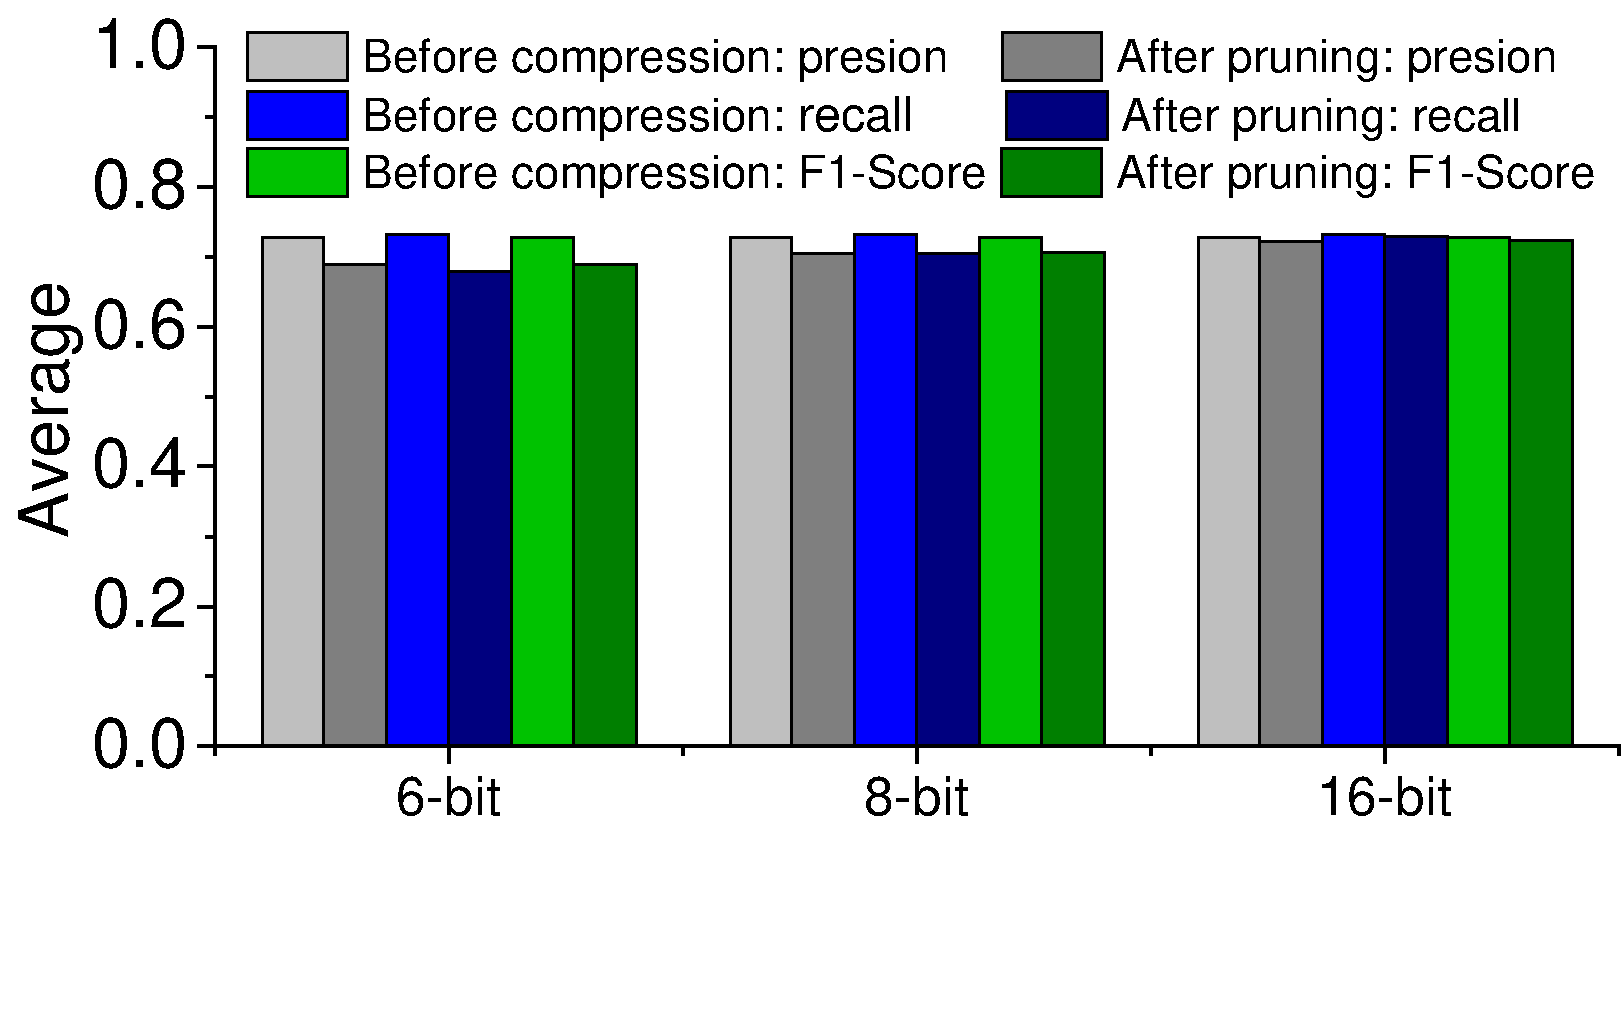
\includegraphics[width=0.33\textwidth]{figure/quan_prf2.pdf}}
\hfill

\caption{The achieved model size (a) inference time (b) accuracy (c) power consumption (d)
energy consumption (e) and precision, recall and F1 score (e) before and after the compression by \quantization.
The compression technique to use depends on the optimization target.}
\label{fig:analy_quan}
\end{figure*}


\begin{figure*}[!t]
\centering
\subfloat[][Model size]{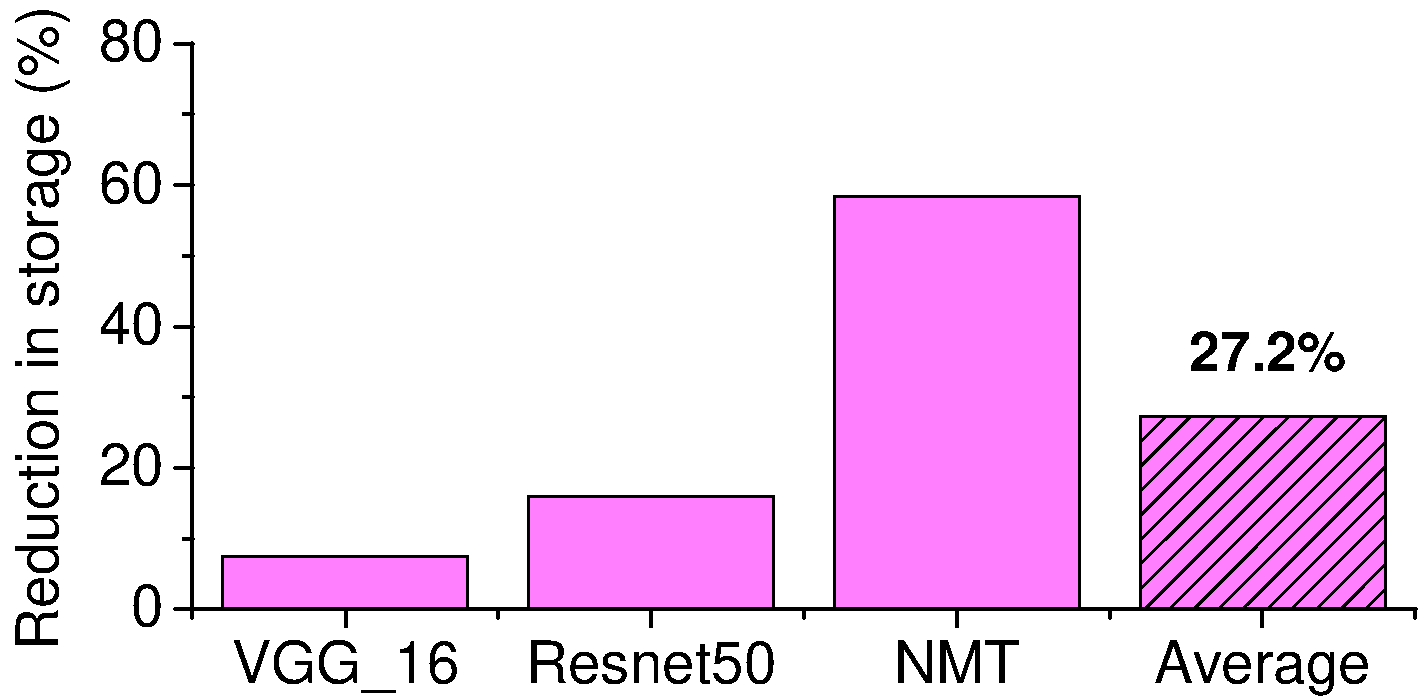
\includegraphics[width=0.33\textwidth]{figure/prun_size.pdf}}
\hfill
\subfloat[][Inference time]{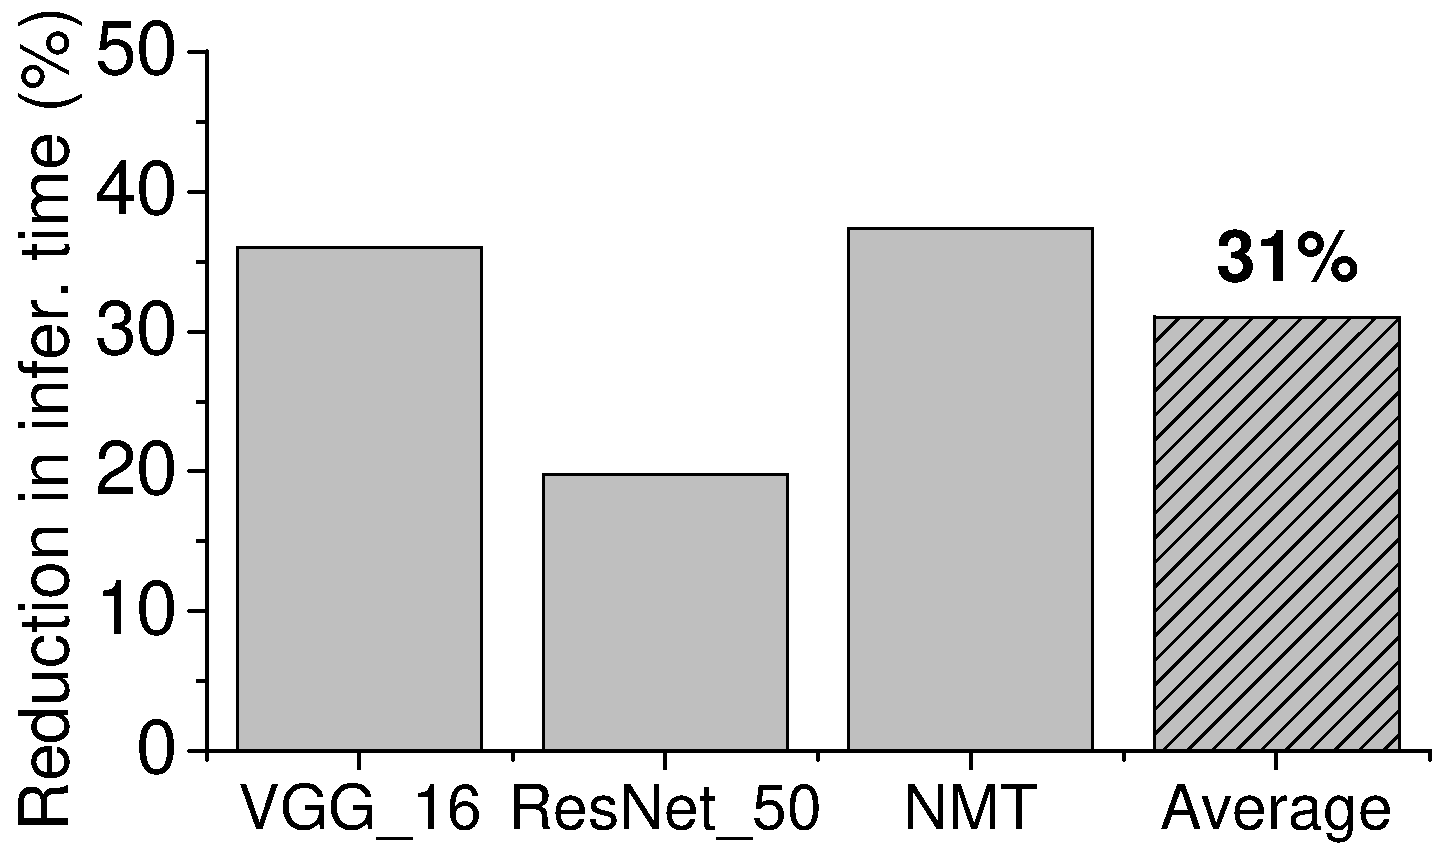
\includegraphics[width=0.3\textwidth]{figure/prun_time.pdf}}
\hfill
\subfloat[][Accuracy]{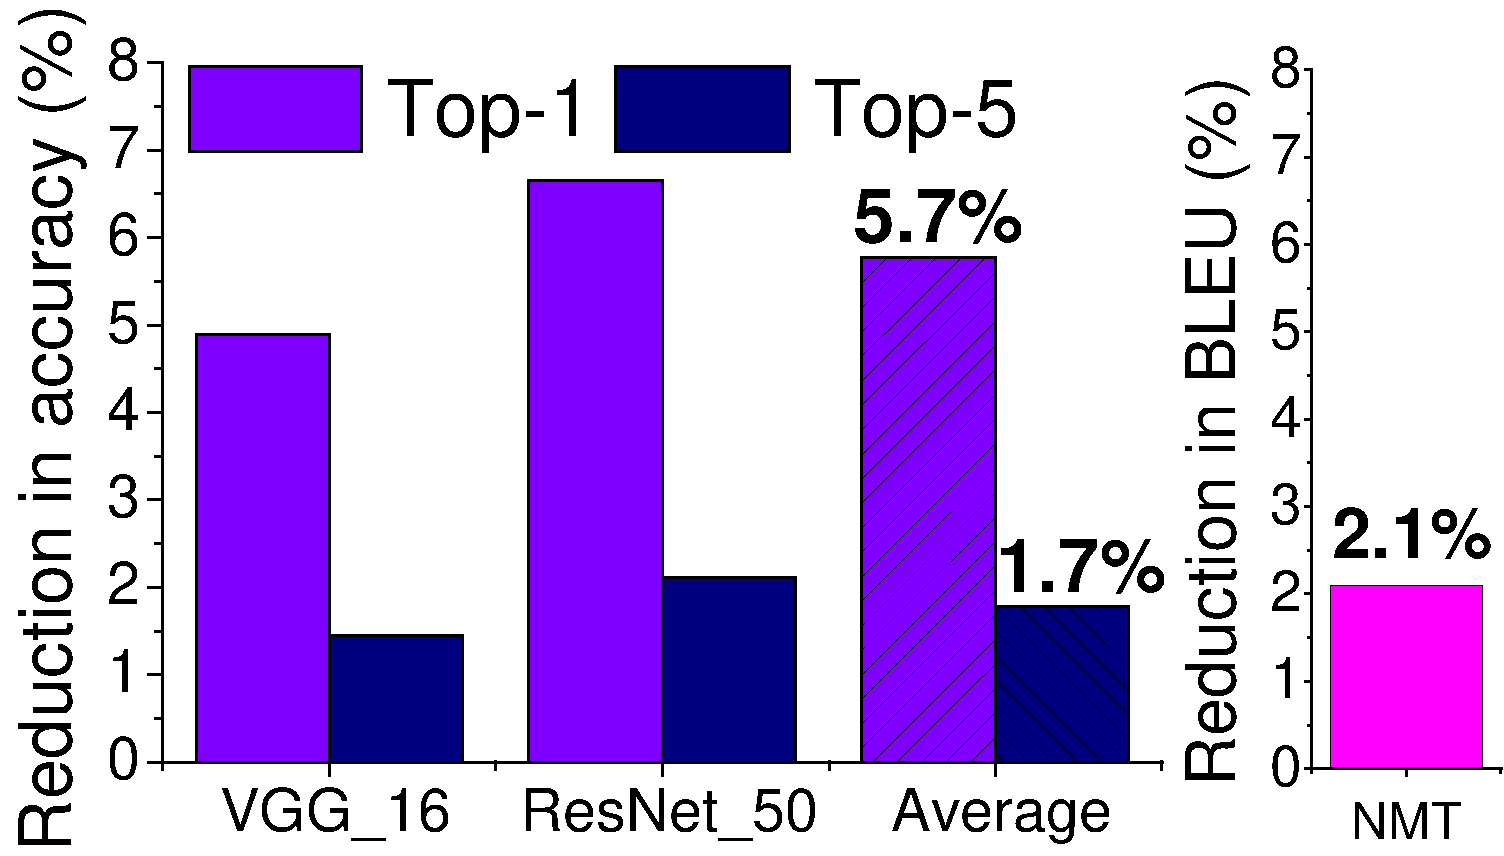
\includegraphics[width=0.3\textwidth]{figure/top1_5_prun.pdf}}
\hfill
\subfloat[][Power consumption]{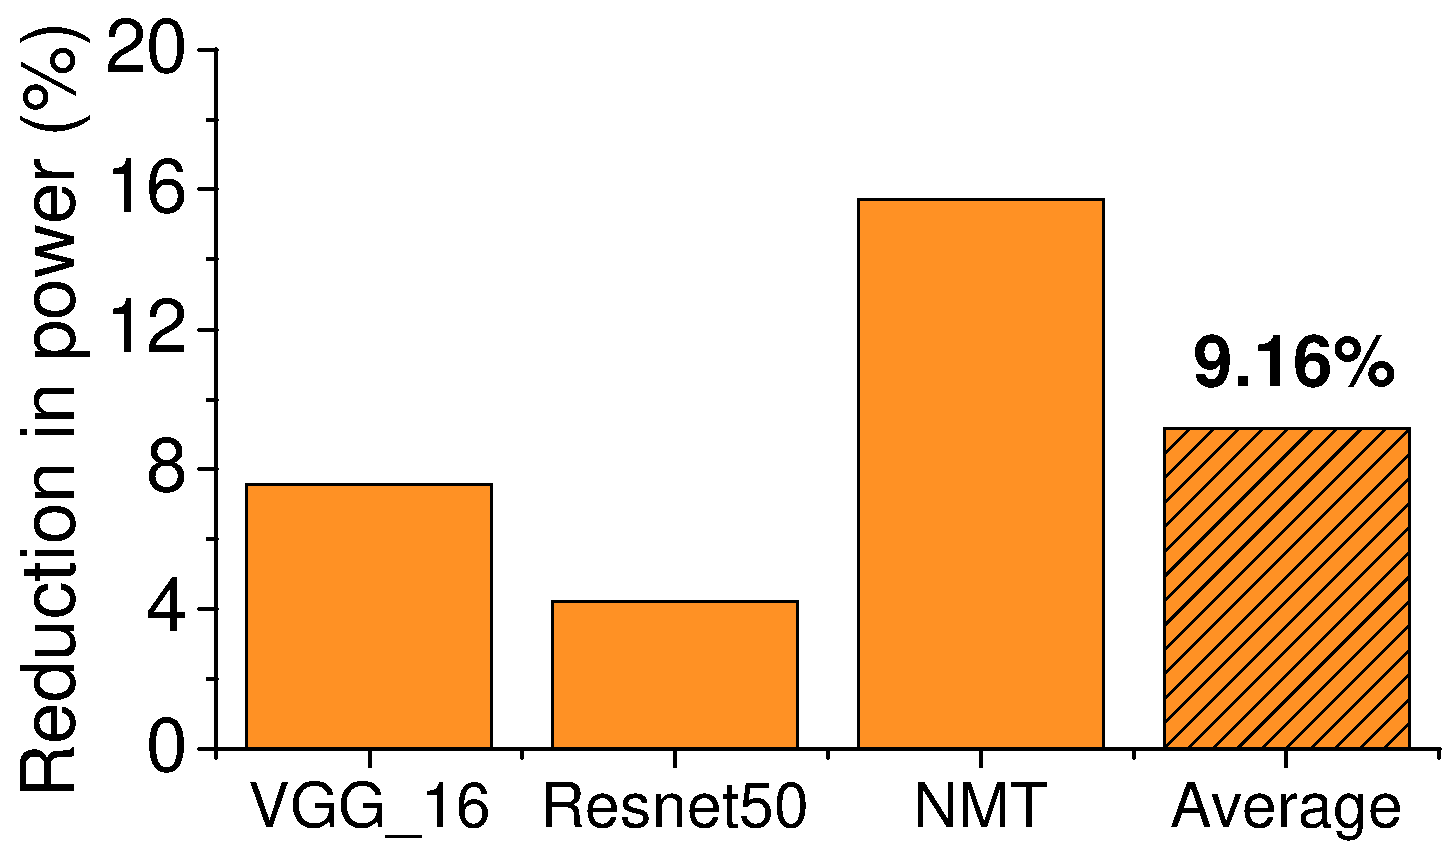
\includegraphics[width=0.3\textwidth]{figure/prun_power.pdf}}
\hfill
\subfloat[][Energy consumption]{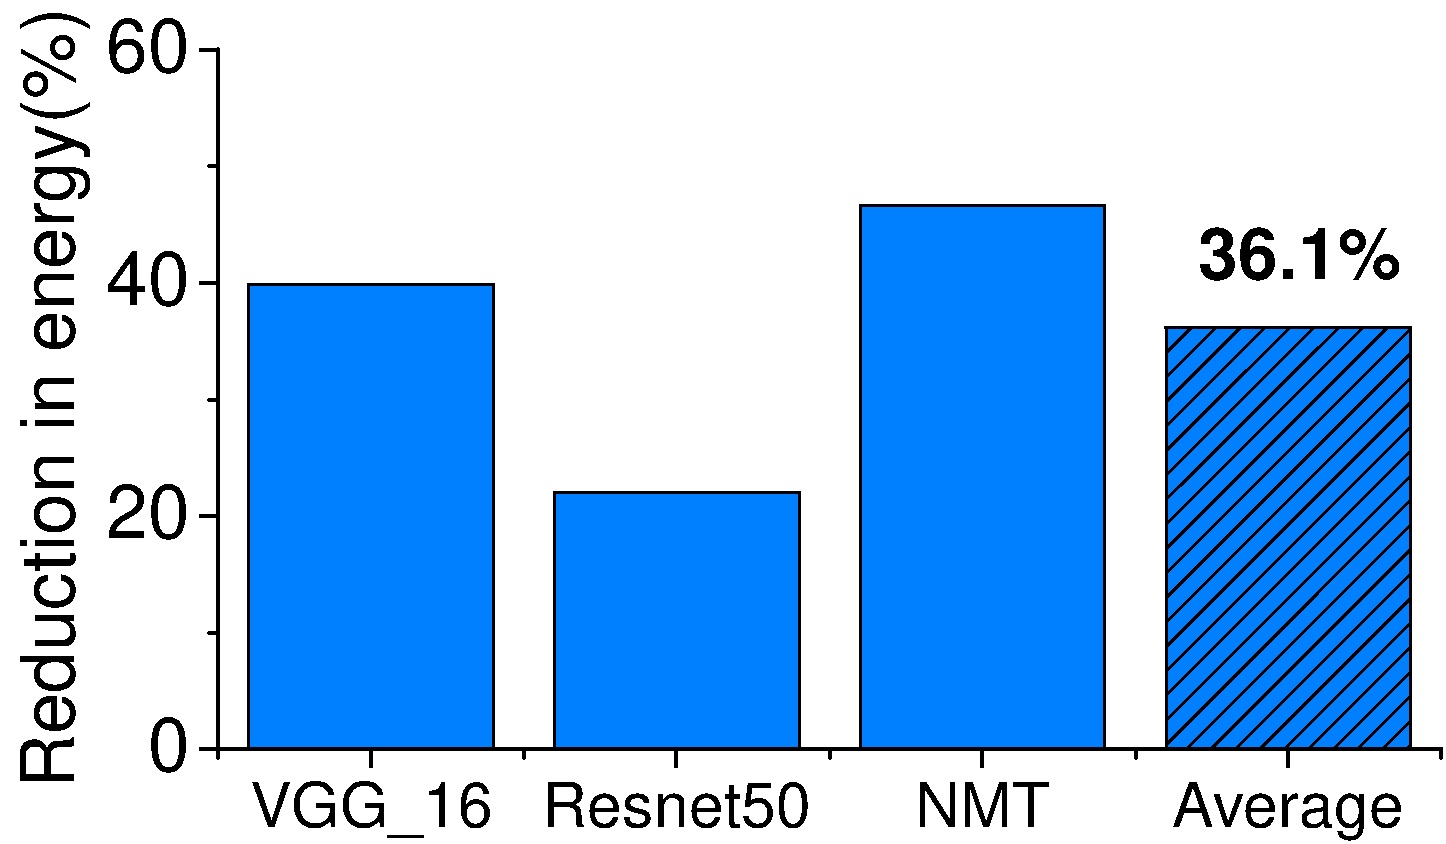
\includegraphics[width=0.3\textwidth]{figure/prun_energy.pdf}}
\hfill
\subfloat[][precision, recall and F1 score]{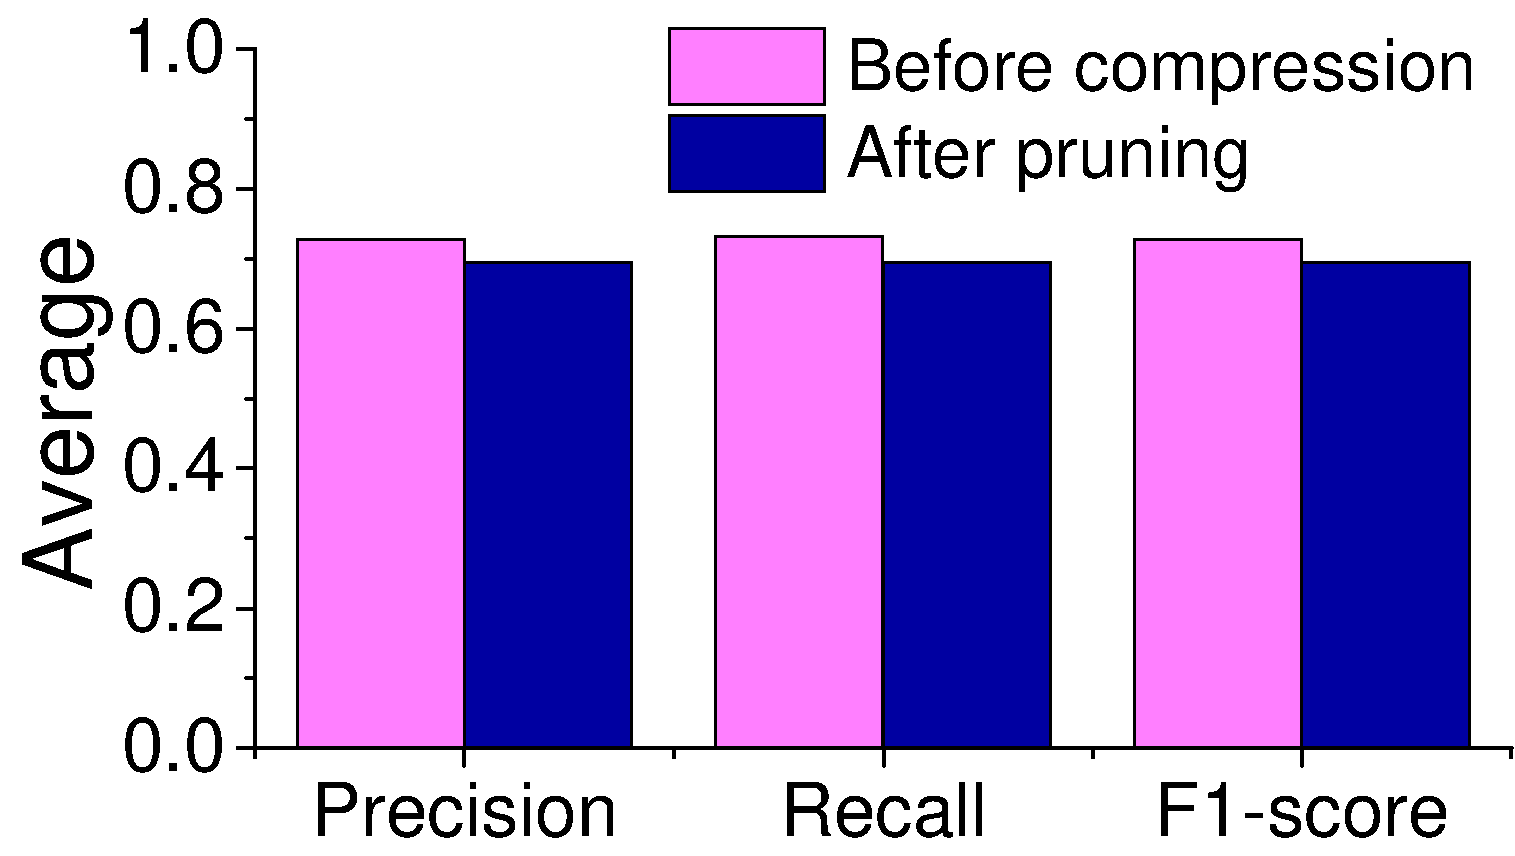
\includegraphics[width=0.3\textwidth]{figure/prun_prf.pdf}}
\hfill

\caption{The change of the model size (a), inference time (b), accuracy/BLEU (c), power (d), energy consumption (e), and accuracy (e)
before and after applying \pruning.} \label{fig:analy_prun}
\end{figure*}

\section{Experimental Results}


\subsection{Roadmap}
Our experiments try to answer the following questions:

\begin{itemize}
\item bla
\item bla2
\item bla3
\end{itemize}

\subsection{Impact on the Model Storage Size\label{sec:ms}}
Reducing the model storage size is crucial for embedded and IoT systems which often have a limited storage space. A smaller model size also
translates to smaller runtime memory footprint of less RAM space consumption. Figures~\ref{fig:analy_quan} and  \ref{fig:analy_prun}
illustrate how the different compression techniques and parameters affect the resulting model size.

As can be seen from Figure~\ref{fig:analy_quan}a, data quantization can significantly reduce the model storage size, leading to an average
reduction of 50.2\% when using a 16-bit representation and up to 80.7\% when using a 6-bit representation. The reduction in the storage
size is consistent across neural networks as the size of a network is dominated by its weights.

From Figure~\ref{fig:analy_prun}a, we see that by removing some of the pathways of the neural network, \pruning can also reduce the model
size, although the gain is smaller than \quantization. On average, \pruning reduces the model size by 27.2\% (49.26 MB). An interesting
observation is that, \pruning is particularly effective for obtaining a compact model for NMT, an \RNN, with a reduction of 60\% on the
model size. This is because there are typically many repetitive pathways in an \RNN due to the natural of the network architecture. As we
will discuss later, \pruning only leads to a minor degradation in the prediction accuracy for NMT. This suggests that \pruning can be an
effective model compression technique for \RNNs.



\subsection{Impact on Inference Time}
 Figure~\ref{fig:analy_quan}b compares the inference time when using different bit
widths to represent a 32-bit floating number for neural network weights. Intuitively, a smaller model should run faster. However, data
quantization does not reduce the inference time but instead it prolongs it. Data quantization can speedup the computation (i.e., matrix
multiplications) performed on the input data by avoiding expensive floating point arithmetics and enabling SIMD vectorization by using a
compact data representation. However, we found that the overhead of the quantization process during inference can outweigh its benefit.
Except the genernal inference operation, a data quantization and de-quantization function has to be added into the compressed model. The quantization function converts the 32-bit to quantized weights, after inference operation which
accounts for 50.9\%, the de-quantization quantized
weights back to a 32-bit representation on the output layer to recover the loss in precision. As can be seen from Figure~\ref{fig:breakdown}, this process could be expensive, contributing to 30\% to 50\% of the end to end inference time.
%this process could be expensive, contributing to 30\% to 50\% of the end to end inference time.
%After data quantization, a de-quantization function has to be added into the compressed model. This  function converts %the quantized
%weights back to a 32-bit representation on the output layer to recover the loss in precision. As can be seen from %Figure~\ref{fig:breakdown},
%this process could be expensive, contributing to 30\% to 50\% of the end to end inference time.

\begin{figure}
\begin{center}
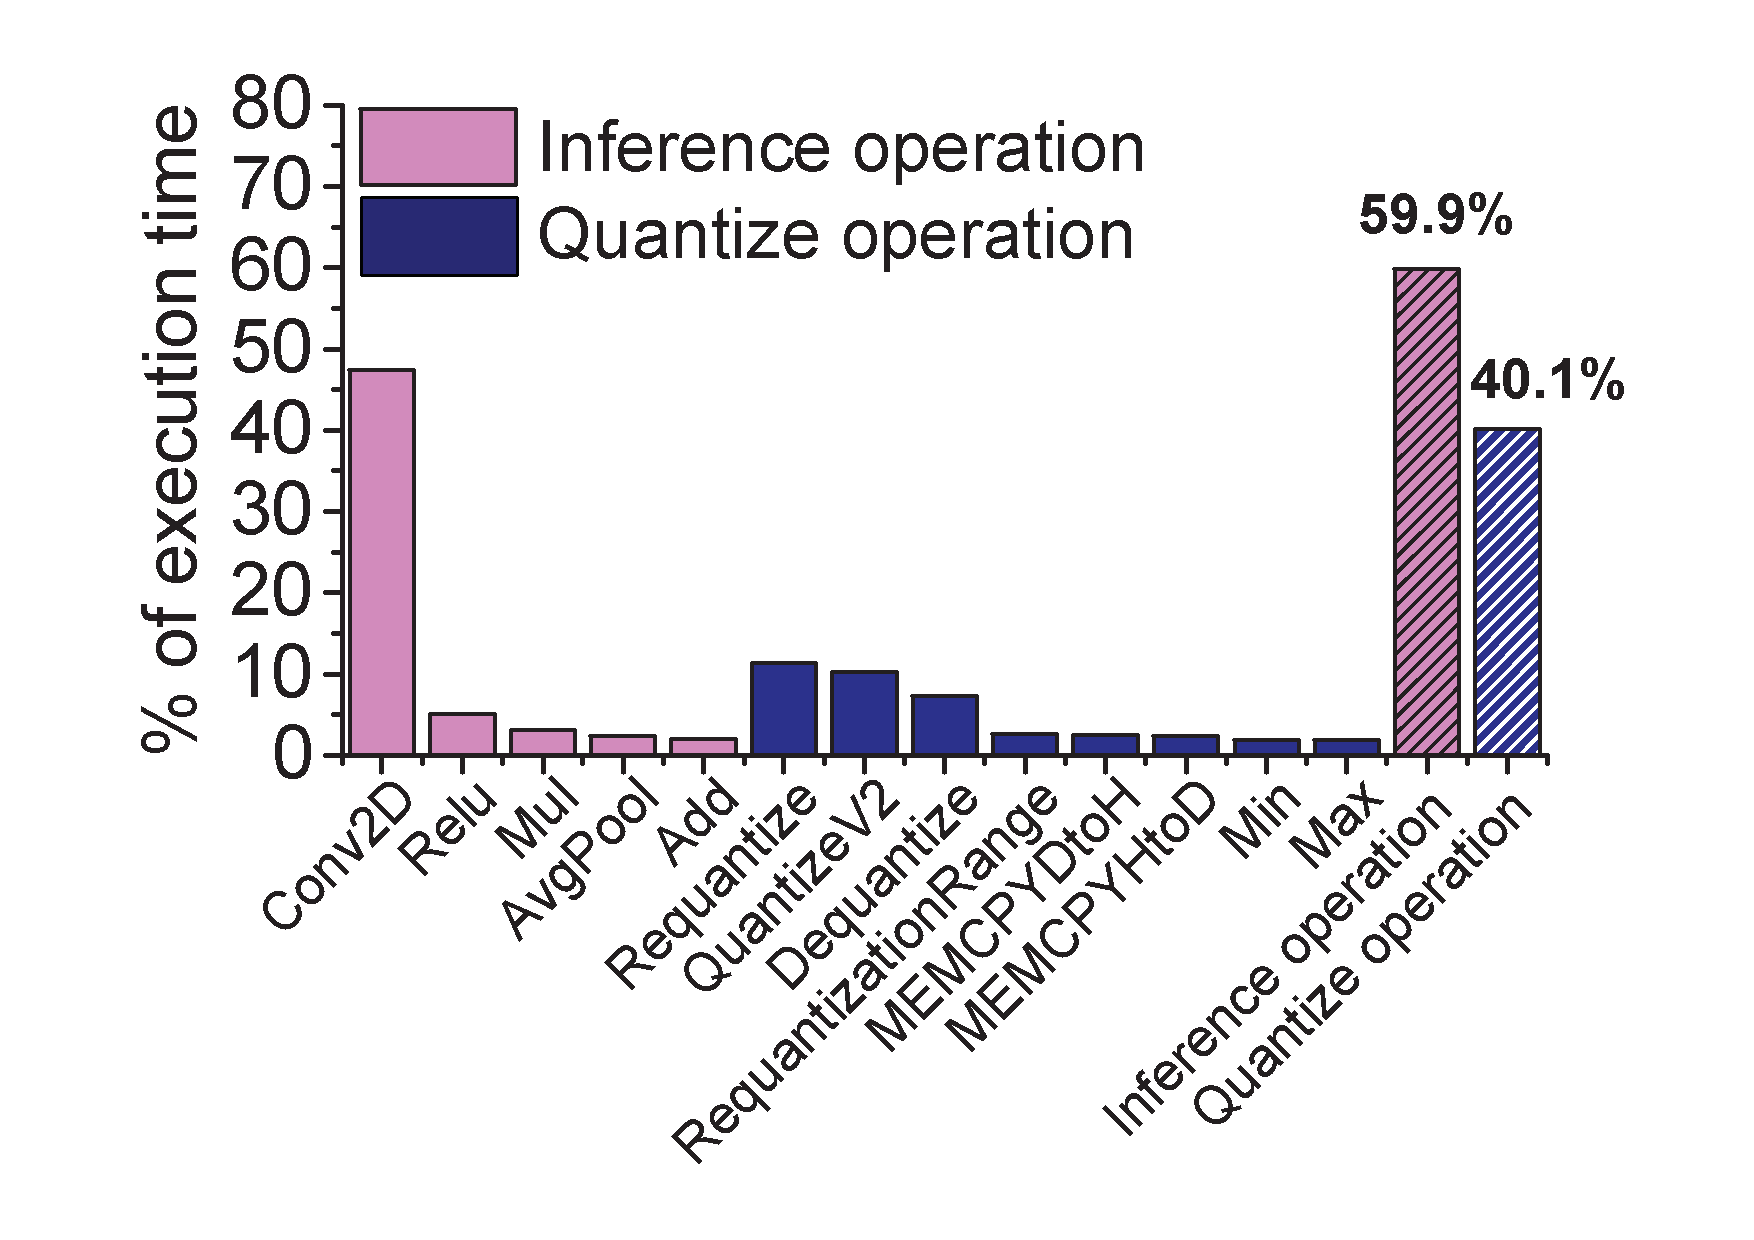
\includegraphics[width=0.48\textwidth]{figure/breakdown2.pdf}
\end{center}
\caption{Breakdown of average execution time by operation type for ten models.}
\vspace{-2mm}
\label{fig:breakdown}
\end{figure}


Using fewer bits for representation can reduce the overhead of de-quantization. For example, using a 6-bit representation is 1.05x and
1.03x faster than using a 16-bit and a 8-bit representations, respectively. However, as we will demonstrate later when discussing
Figure~\ref{fig:analy_quan}c, using fewer bits has the drawback of causing larger degradation in the prediction accuracy. Hence, one must
carefully find a balance between the storage size, inference time, and prediction accuracy when applying data quantification.

We also find that the percentage of increased inference time depends on the neural network structure. Applying data quantization to
\texttt{Inception}, the most complex network in our \CNN tested set, will double the inference time. By contrast, data quantization only
leads to a 20\% increase in inference time for \texttt{Mobilenet}, a compact model. This observation suggests that data quantization may be
beneficial for simple neural networks on resource-constrained devices.


In contrast to \quantization, Figure~\ref{fig:analy_prun}b shows that \pruning leads to faster inference time across evaluated networks. We
can see that the inference time of \texttt{Vgg\_16} and \texttt{NMT} can benefit from this technique, with an reduction of 38\%.  Overall,
the average inference time is reduced by 31\%. This suggests that while \pruning is less effective in reducing the model size (see
Section~\ref{sec:ms}), it can be useful in achieving a faster inference time.


\subsection{Impact on Accuracy Metrics}
In addition to the storage size and inference time, accuracy is crucially important for a predictive model. A small and faster model is not
very useful if it gives wrong predictions all the time.


Results in Figure~\ref{fig:analy_quan}c compare how the prediction accuracy is affected by model compression. We see that the sweat spot of
\quantization depends on the neural network structure. An 16-bit representation keeps the most information of the original model and thus
leads to little reduction in the prediction accuracy, on average  1.36\%.  Using an 8-bit representation would lead on average 3.57\%
decrease in the accuracy, while using a 6-bit representation will lead to a significantly larger reduction of 10\% in  accuracy. We also
observe that some networks are more robust to \quantization. For example, while a 6-bit representation leads to less than 10\% decrease in
accuracy for \texttt{Resnet\_101}, it cause a 12\% drops in accuracy for \texttt{Resnet\_50}. This is because a more complex network (i.e.,
\texttt{Resnet\_101} in this case) is more resilient to the weight errors compared to network (i.e., \texttt{Resnet\_50} in this case) with
a smaller number of layers and neurons. Our findings suggest the need for having an adaptive scheme to choose the optimal \dquantization
parameter for given constraints.


For \pruning, the Figure~\ref{fig:analy_prun}c compares the reduction in the top-1 and the top-5 accuracies for \texttt{Vgg\_16} and
\texttt{Resnet\_50}. We also show the BLEU value for \texttt{NMT}. \pruning reduces the accuracy of the two \CNN models with by 5.7\% and
1.7\% respectively for the top-1 and top-5 scores. We observe that the \pruning has little negative impact on \texttt{NMT} where we only
observe an averaged loss of 0.8\% for BLEU. When taking into consideration that \pruning can significantly reduce the model size for
\texttt{NMT} (Section~\ref{sec:ms}), our results suggest that \pruning is particularly effective for \RNNs.


%Although an 8-bit representation leads to a minor
%decrease in the prediction accuracy, a further reduction of a 6-bit representation is only profitable for xx networks.



\subsection{Impact on the Power and Energy Consumption}
Power and energy consumption are two limiting factors on battery-powered mobile and IoT devices. As we can see from
Figure~\ref{fig:analy_prun}d, \quantization decreases the peak power for inferencing with an average of 4.3\%, 10.4\% and 11.6\%,
respectively when using a 6-bit, an 8-bit and a 16-bit representations. While \quantization reduces the peak power used, the increase
inference time leads to more energy consumption by at least 34.1\% and up to 51.1\% (see Figure~\ref{fig:analy_prun}e). This means that
although \quantization allows one to reduces voltage supply to the computing devices, it can lead to a short battery life.

Figure~\ref{fig:analy_prun}e shows the reduced energy consumption by applying \pruning. Note that it saves over 40\%, 15\% and 50\% energy
consumption for \texttt{Vgg\_16}, \texttt{Resne\_50} and \texttt{NMT} respectively. Despite that the peak power is reduced by only 9.16\%,
a smaller decrease compared to \quantization, the resulted faster inference time allows \pruning to significantly reduce the power
consumption. The results suggest \pruning is useful for reducing the overall energy consumption of the system, but \quantization can be
employed to support a low power system.



\subsection{Precision, Recall and F1-Score}

Finally, Figure~\ref{fig:analy_quan}f and 
Figure~\ref{fig:analy_prun}f show other three evaluation metrics of these models 
after \quantization and \pruning. We can see that, the compressed models only violate
less than 3\% for precision, recall and F1-Score. 
For \quantization, the 16-bit representation outperforms the other two bits width respresentations.
Specifically, 16-bit gives the
highest overall precision, which in turns leads to the best F1
score. High precision can reduce false positive, which is
important for certain domains like video surveillance
because it can reduce the human involvement for inspecting
false positive predictions.




\subsection{Memory footprint}

\begin{figure}[!t]
\centering
\subfloat[][\quantization]{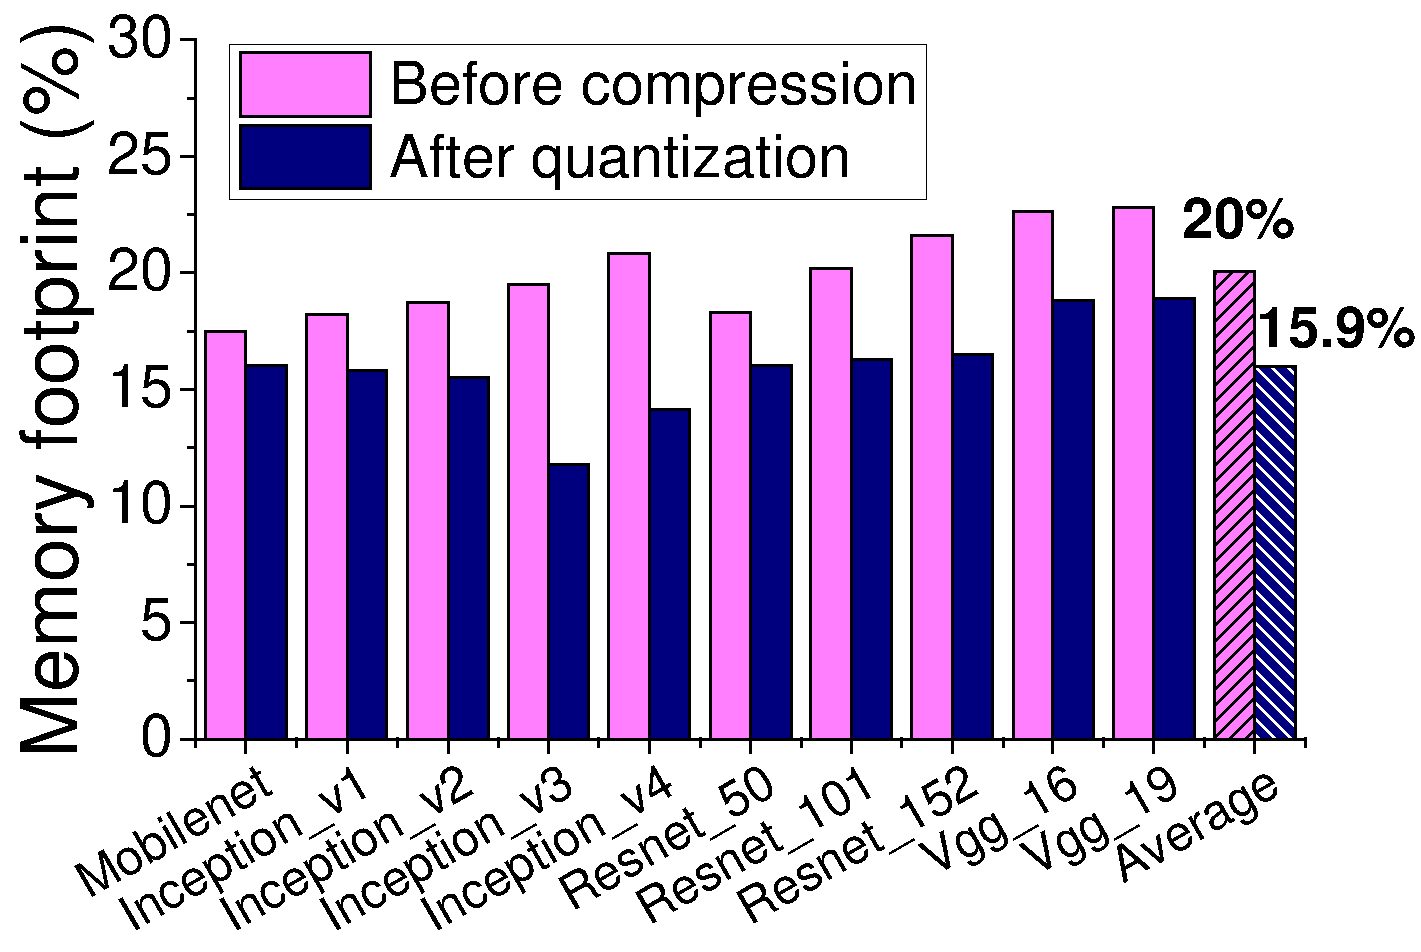
\includegraphics[width=0.4\textwidth]{figure/quan_mem.pdf}}
\hfill
\subfloat[][\pruning]{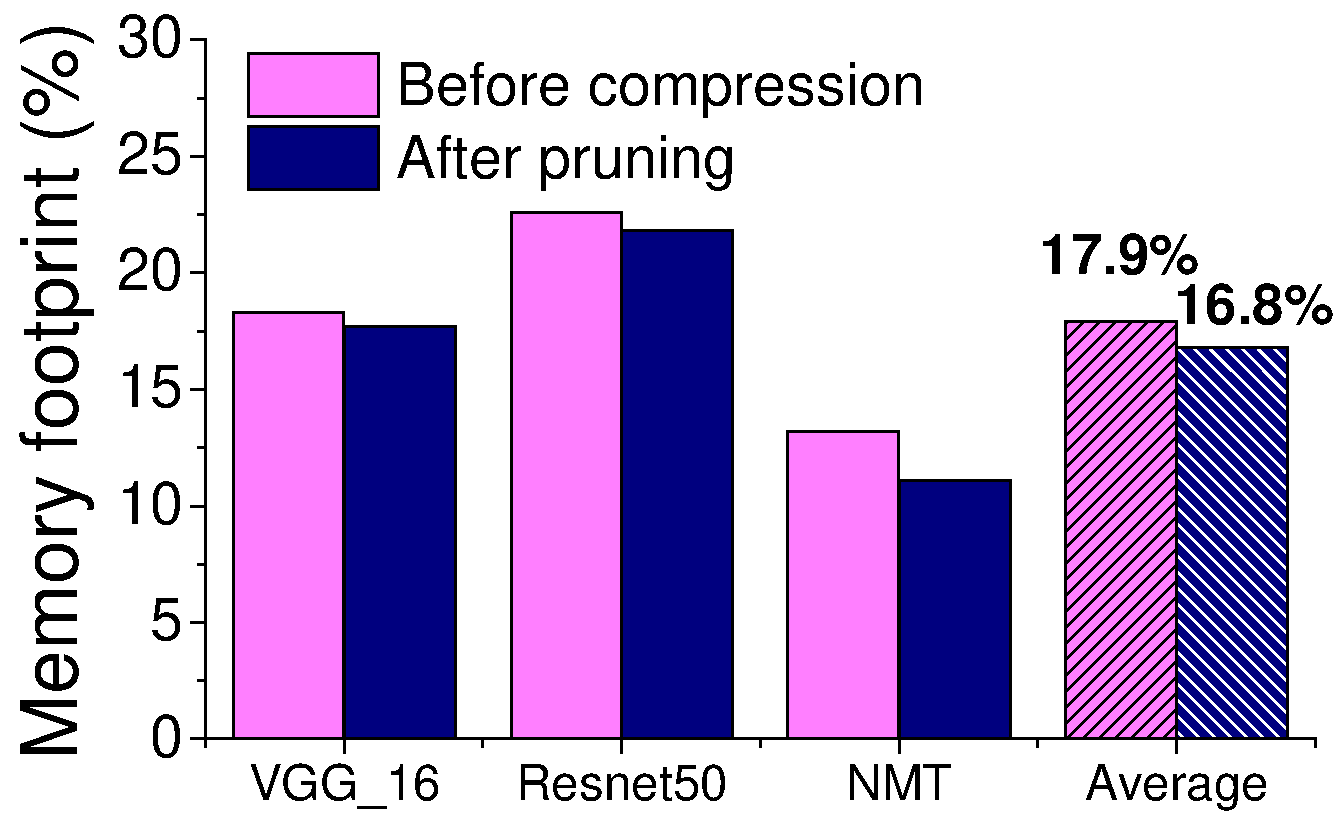
\includegraphics[width=0.4\textwidth]{figure/prun_mem.pdf}}
\hfill

\caption{Memory footprint before and after the compression by \quantization(a) and \pruning (b).}
\label{fig:footprint}
\end{figure}

Figure~\ref{fig:footprint} compares the resulting memory footprint by applying \quantization and \pruning. Quantization reduces the runtime
memory footprint with an averaged reduction of 17.2\% by generating a more compact model. For example, an 8-bit representation reduces the
memory footprint from 20.02\% to 15.97\% across networks, with an averaged reduction of 20.63\% (up to 40\%). In general, the smaller the
model storage size is, the less memory footprint the compressed model will be. As an example, a 6-bit representation uses \FIXME{xx, and
xx} less memory compared to a 8-bit and a 16-bit representations, respectively.

In contrast to \dquantization, Figure~\ref{fig:footprint} shows that  \pruning offers little help in reducing the model memory footprint.
On average, it leads to a 6.4\% reduction of memory footprint. This is because that the network weights still domain the memory resource
consumption, and \pruning is less effective compared to \dquantization for reducing the overhead of network weights.


\subsection{Compare to Oracle.} 

\begin{figure}[!t]
\centering

\subfloat[][\quantization]{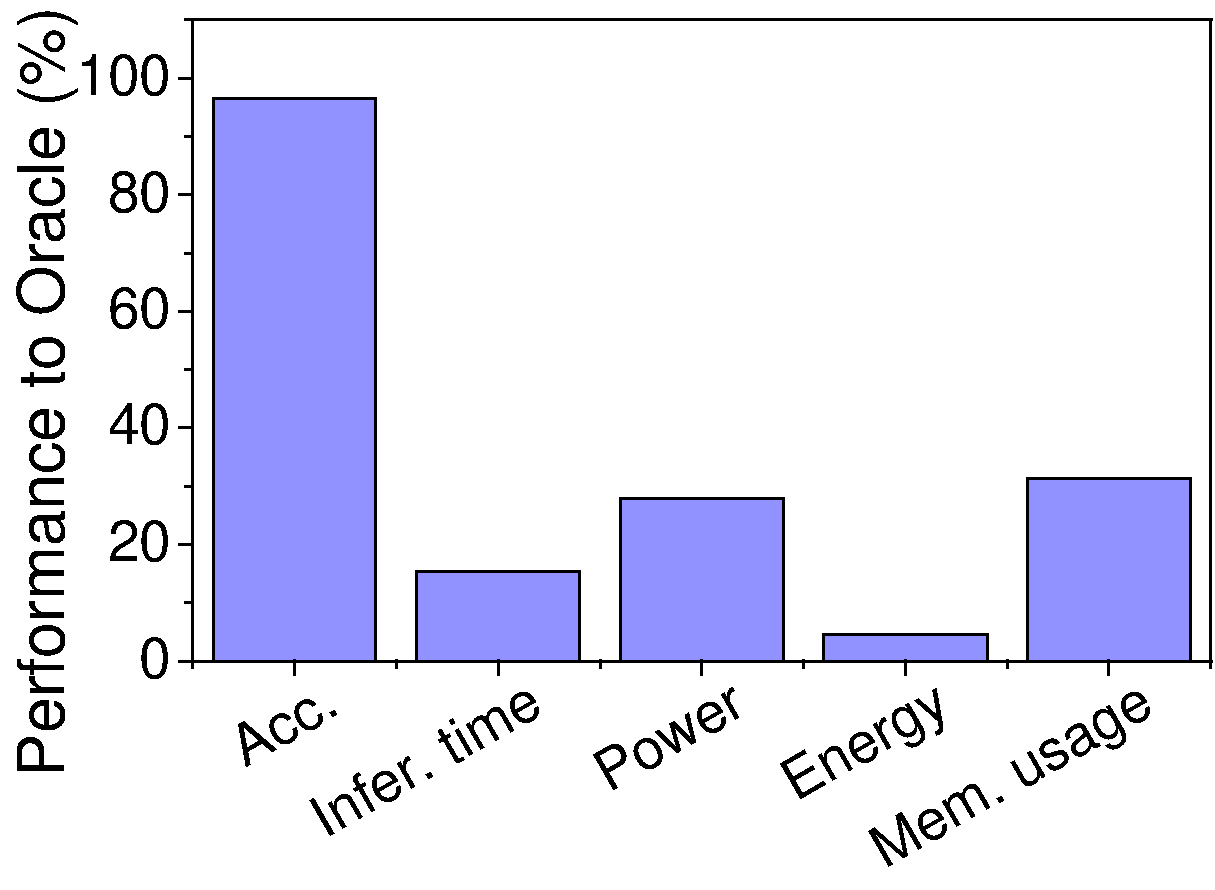
\includegraphics[width=0.35\textwidth]{figure/quan_oracle.pdf}}
\hfill
\subfloat[][\pruning]{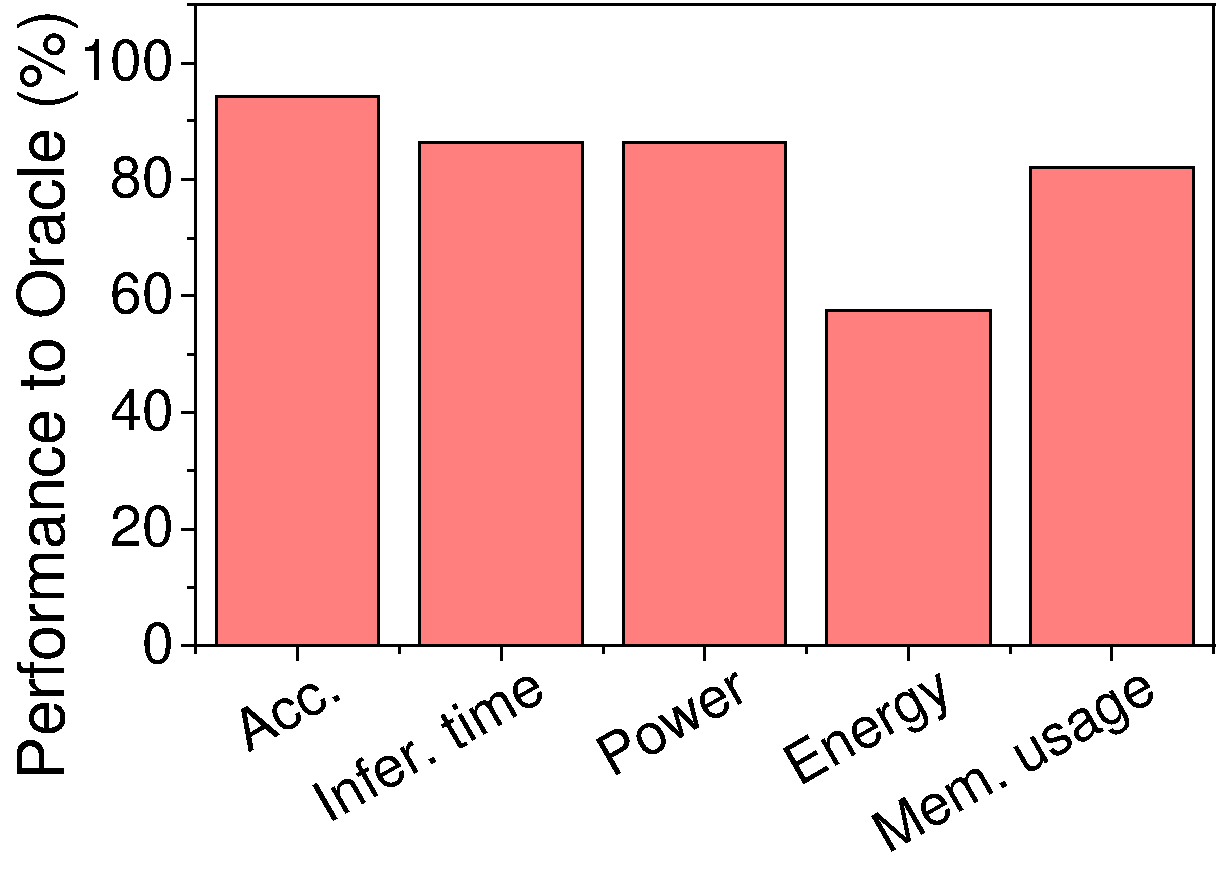
\includegraphics[width=0.35\textwidth]{figure/prun_oracle.pdf}}
\hfill

\caption{Our compressed models' performance w.r.t. performance of an oracle performance for \quantization (a) and \pruning (b).}
\label{fig:oracle}
\end{figure}

In Figure~\ref{fig:oracle}, we compare our compressed models to ideal compressed models. 
We set the 8-bit data quantization as the ideal quantized weight, as it offers an affordable 
accuracy after quantization. Note that, the accuarcy almost achieves the ideal value, on the contary,
the inference time and enery consumption perform worst, only account less than 10\%. Bot of 
the inference time and memory usage occupy more than 20\%.
Figure~\ref{fig:oracle} b presents the how close our pruned models to the theoretically 
perfect models. As we can see from this figure, most of evaluation metrics above 80\%,
and the energy consunsumption also achieves 58\%.





\section{Related Work}
\DNNs have shown astounding successes in various tasks that previously seemed difficult~\cite{}. Despite the fact that many embedded
devices require precise sensing capabilities, adoption of \DNN models on such systems has notably slow progress. This mainly due to
\DNN-based inference being typically a computation intensive task, which inherently runs slowly on embedded devices due to limited
resources.

\FIXME{Talk about different compression techniques.}

There is an extensive body of work on how to accelerate \DNN training using xx, xx, and xx. Our work aims to understand how to accelerate
deep learning inference by choosing the right model compression technique.


As an alternative to on-device inferencing, off-loading computation to the cloud can accelerate \DNN model inference
\cite{teerapittayanon2017distributed}. Neurosurgeon \cite{Kang2017neurosurgeon} identifies when it is beneficial (\eg in terms of energy
consumption and end-to-end latency) to offload a \DNN layer to be computed on the cloud. The Pervasive \CNN~\cite{7920809} generates
multiple computation kernels for each layer of a \CNN, which are then dynamically selected according to the inputs and user constraints. A
similar approach presented in \cite{RodriguezWZMH17} trains a model twice, once on shared data and again on personal data, in an attempt to
prevent personal data being sent outside the personal domain. Computation off-loading is not always applicable due to privacy, latency or
connectivity issues. The work presented by Ossia \etal partially addresses the issue of privacy-preserving when offloading \DNN inference
to the cloud ~\cite{ossia2017hybrid}. Our work is complementary to prior work on computation off-loading by offering insights to choose the
optimal compression technique to best optimize local inference.

\section{Conclusions}
This paper has presented an automatic approach to optimize the mobile web



\bibliographystyle{plain}
\bibliography{refs}


\end{document}
